\documentclass[8pt,spanish]{beamer}
% Compilar con: lualatex -shell-escape dl_2h_presentation.tex
% ---------------------------------------------------------
% PACKAGES -------------------------------------------------
\usepackage{fontspec}          % Fuente Unicode (lualatex)
\setsansfont{Fira Sans}
\setmonofont{Fira Mono}
\usepackage{minted}            % Código con resaltado
\usepackage{graphicx}          % Figuras
\usepackage{mwe}               % Imágenes de ejemplo -> example-image
\usepackage{hyperref}          % Vínculos clicables
\hypersetup{colorlinks=true, urlcolor=blue}
\usepackage{booktabs}          % Tablas bonitas
\usepackage{babel}
\usepackage{verbatim}
\usepackage{tikz}

\usepackage{booktabs}   % \toprule, \midrule, \bottomrule
\usepackage[table]{xcolor} % colors + \rowcolors
\usepackage{tabularx}   % flexible column widths
\renewcommand{\arraystretch}{1.15} % airy vertical spacing

% CONFIGURACIÓN DE MINTED ---------------------------------
\setminted{
    linenos,
    fontsize=\footnotesize,
    breaklines,
    tabsize=2,
    frame=lines
}

% TEMA DE BEAMER ------------------------------------------
\usetheme{Madrid}
\usecolortheme{default}
\definecolor{dlblue}{HTML}{003f5c}
\setbeamercolor{structure}{fg=dlblue}

% METADATOS ------------------------------------------------
\title{\textbf{Esenciales de Deep Learning}}
\subtitle{Presentación intensiva de 2 horas}
\author{J. Peralta}
\institute{Universidad Andrés Bello}
\date{Julio 2025}

% ----------------------------------------------------------
\begin{document}

% PORTADA --------------------------------------------------
\begin{frame}
  \titlepage
\end{frame}

% ÍNDICE ---------------------------------------------------
\begin{frame}{Guía de la sesión}
  \tableofcontents
\end{frame}


% ==========================================================
\section{IA, ML y Deep Learning}
% ----------------------------------------------------------
% 1. Mapa conceptual
\begin{frame}{Mapa conceptual}
  \centering
  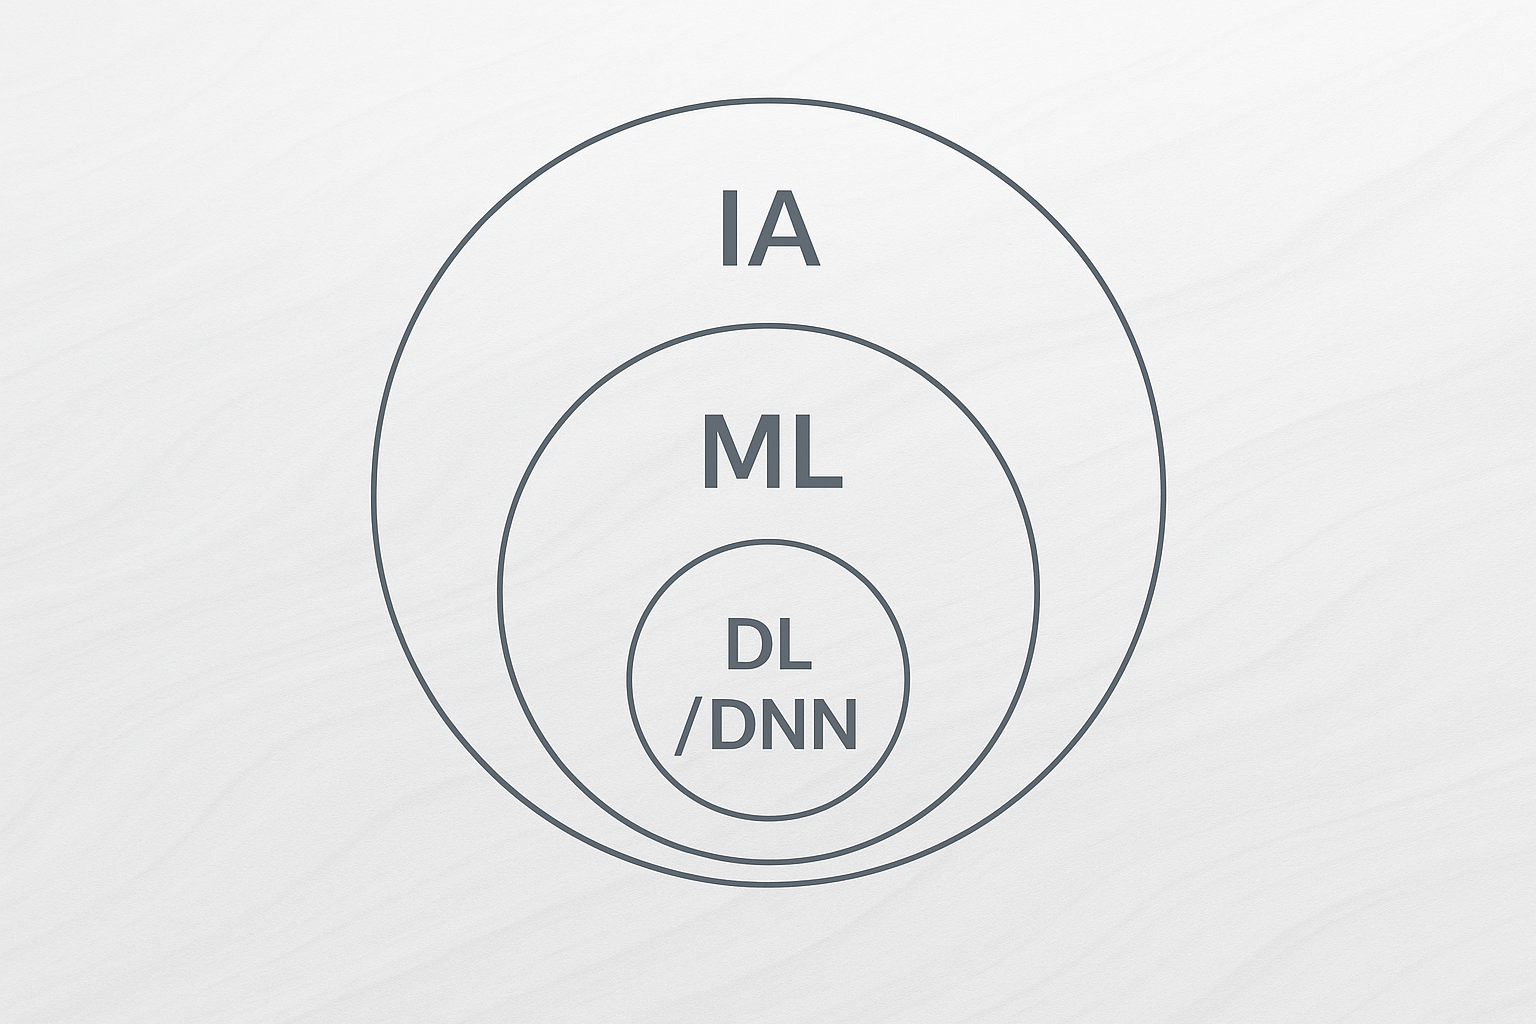
\includegraphics[width=.5\textwidth]{Concept-1.png}
  %\vspace{.5em}

  \begin{itemize}
    \item \textbf{IA} engloba cualquier técnica que emule comportamientos inteligentes.
    \item \textbf{ML} aprende patrones a partir de datos; es un subconjunto de IA.
    \item \textbf{DL / DNN} aprende representaciones jerárquicas con redes profundas;
      es un subconjunto de ML.
  \end{itemize}
\end{frame}

%----------------------------------------------------------------------%
% 2. Inteligencia Artificial
%----------------------------------------------------------------------%
\begin{frame}[fragile]{¿Qué entendemos por Inteligencia Artificial?}

\begin{columns}[T]
%--------- Left column -------------------------------------------------%
\begin{column}{0.55\textwidth}
  \begin{itemize}
    \item \textbf{Tareas clásicas}:  
      \begin{itemize}
        \item \alert{Razonamiento} → demostradores de teoremas (\textit{Prover9}).  
        \item \alert{Planificación} → rover \textit{Sojourner} (NASA, 1997).  
        \item \alert{Percepción} → detección de peatones en vehículos autónomos.  
        \item \alert{Procesamiento de lenguaje} → ChatGPT, traducción automática.  
      \end{itemize}
    \item \textbf{Paradigmas históricos}:
      \begin{itemize}
        \item \textbf{GOFAI} (reglas \texttt{IF–THEN}, lógica de predicados, MYCIN).  
        \item \textbf{Búsqueda} (A*, Minimax + αβ; \textit{Deep Blue}, 1997).  
        \item \textbf{Probabilístico} (redes bayesianas, POMDP).  
      \end{itemize}
    \item \textbf{Éxitos tempranos}: diagnóstico médico, ajedrez, planificación de satélites.  
  \end{itemize}

  \begin{block}{Clave}
    No toda IA \emph{aprende}; muchos sistemas se basan en reglas codificadas a mano.
  \end{block}
\end{column}

%--------- Right column ------------------------------------------------%
\begin{column}{0.45\textwidth}
  \begin{center}
    %-- Diagrama de contención IA ⊃ ML ⊃ DL ----------------------------%
    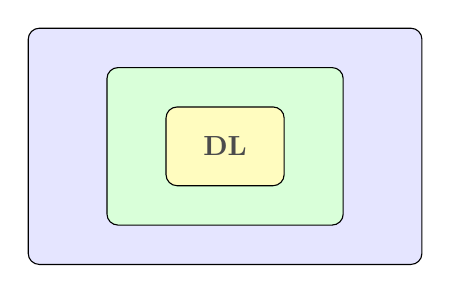
\begin{tikzpicture}[every node/.style={font=\small}]
      % IA
      \draw[fill=blue!10, rounded corners] (0,0) rectangle (5,3)
        node[pos=.5,font=\bfseries\Large,black!70] {IA};
      % ML
      \draw[fill=green!15, rounded corners] (1,0.5) rectangle (4,2.5)
        node[pos=.5,font=\bfseries,black!70] {ML};
      % DL
      \draw[fill=yellow!25, rounded corners] (1.75,1) rectangle (3.25,2)
        node[pos=.5,font=\bfseries,black!70] {DL};
    \end{tikzpicture}

    \vspace{0.6em}
    %-- (Opcional) Foto histórica Deep Blue vs Kasparov -----------------%
    % \includegraphics[width=\linewidth]{deep_blue_kasparov.jpg}\\
    % {\tiny Garry Kasparov vs Deep Blue, 11 mayo 1997}
  \end{center}
\end{column}
\end{columns}
\end{frame}

%----------------------------------------------------------------------%
% 3. Machine Learning
%----------------------------------------------------------------------%
\begin{frame}[fragile]{Machine Learning: aprender de los datos}

\begin{columns}[T]
%--------- Left column -------------------------------------------------%
\begin{column}{0.43\textwidth}
  \begin{itemize}\small
    \item \textbf{Objetivo}: construir modelos que \emph{generalicen} a partir de datos.
    \item \textbf{Paradigmas fundamentales}:
      \begin{description}\footnotesize
        \item[Supervisado:] clasificación (\textit{spam / no-spam}), regresión (predicción de demanda eléctrica).
        \item[No supervisado:] \textit{k}-means en catálogos galácticos,  reducción de dimensionalidad (t-SNE en MNIST).
        \item[Por refuerzo:] AlphaGo, control de drones, trading algorítmico.
      \end{description}
    \item \textbf{Algoritmos clásicos}:  
      Regresión lineal, \(k\)-NN, Árboles y Bosques Aleatorios, SVM, \textit{k}-means.
    \item \textbf{Tendencias recientes}: AutoML, aprendizaje federado en dispositivos móviles.
  \end{itemize}
\end{column}

%--------- Right column ------------------------------------------------%
\begin{column}{0.53\textwidth}
  \begin{center}
    %-- Diagrama de ciclo RL -------------------------------------------%
    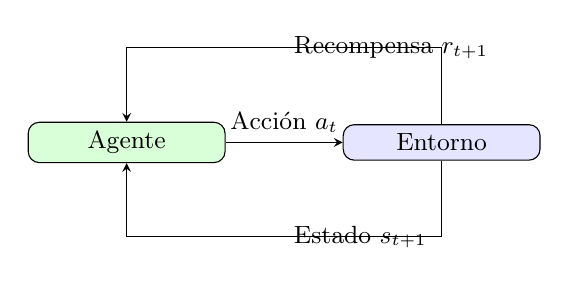
\begin{tikzpicture}[>=stealth, node distance=2.3cm, every node/.style={font=\small}]
      \node[draw, rounded corners, fill=green!15, minimum width=2.5cm] (agent) {Agente};
      \node[draw, rounded corners, fill=blue!10, right of=agent, xshift=1.7cm,
            minimum width=2.5cm] (env) {Entorno};
      \draw[->] (agent) -- node[above]{Acción \(a_t\)} (env);
      \draw[->] (env) -- ++(0,-1.2) -| node[pos=0.25,right]{Estado \(s_{t+1}\)} (agent);
      \draw[->] (env) -- ++(0,1.2) -| node[pos=0.25,right]{Recompensa \(r_{t+1}\)} (agent);
    \end{tikzpicture}

    \vspace{1.1em}
    %-- (Opcional) Imagen SVM ------------------------------------------%
    % \includegraphics[width=\linewidth]{svm_margin_example.png}\\
    % {\tiny Hiperplano separador con SVM}
  \end{center}
\end{column}
\end{columns}
\end{frame}


% 4. Deep Learning & DNN
\begin{frame}{Deep Learning y redes neuronales profundas}
  \begin{itemize}
    \item Redes con muchas capas (+ millones de parámetros) que aprenden
          representaciones jerárquicas.
    \item Arquitecturas: CNN, RNN/LSTM, Transformers, GNN.
    \item Escalan bien con grandes volúmenes de datos y potencia GPU/TPU.
  \end{itemize}
  \begin{block}{Observación}
    DL = representación + aprendizaje \(\Rightarrow\) elimina ingeniería manual de características.
  \end{block}
\end{frame}

% 5. Tabla comparativa
\begin{frame}[fragile]{Comparativa IA vs ML vs DL}
  \begin{center}
    {\Large
    % Modern comparison table (place inside your frame or center environment)
\rowcolors{2}{gray!5}{white}        % subtle zebra striping
\begin{tabularx}{\linewidth}{>{\bfseries}l *{3}{>{\centering\arraybackslash}X}}
\toprule
Aspecto & IA & ML & DL\\
\midrule
Datos necesarios    & Bajo–medio & Medio & Alto\\
Ingeniería manual   & Alta       & Media & Baja\\
Interpretabilidad   & Alta       & Media & Baja\\
Hardware            & CPU        & CPU/GPU & GPU/TPU\\
Tareas típicas      & Planificación & Predicción & Visión, lenguaje\\
\bottomrule
\end{tabularx}

    }
  \end{center}
\end{frame}

% 6. Código ilustrativo
\begin{comment}
\begin{frame}[fragile]{De la regresión lineal a una DNN en 10 líneas}
  \begin{minted}[fontsize=\footnotesize]{python}
# Regresión lineal clásica (scikit-learn)
from sklearn.linear_model import LinearRegression
model = LinearRegression().fit(X_train, y_train)

# Misma tarea con Keras (DNN pequeña)
from tensorflow.keras import Sequential, layers
dnn = Sequential([
    layers.Dense(64, activation='relu', input_shape=(X_train.shape[1],)),
    layers.Dense(1)
])
dnn.compile(optimizer='adam', loss='mse')
dnn.fit(X_train, y_train, epochs=50, batch_size=32)
  \end{minted}
  \vspace{-1em}
  \begin{itemize}
    \item \textbf{DL} reemplaza el mapeo lineal por capas no lineales aprendidas.
  \end{itemize}
\end{frame}

\end{comment}

% 7. Datos vs Rendimiento
\begin{frame}{Rendimiento vs cantidad de datos}
  \centering
  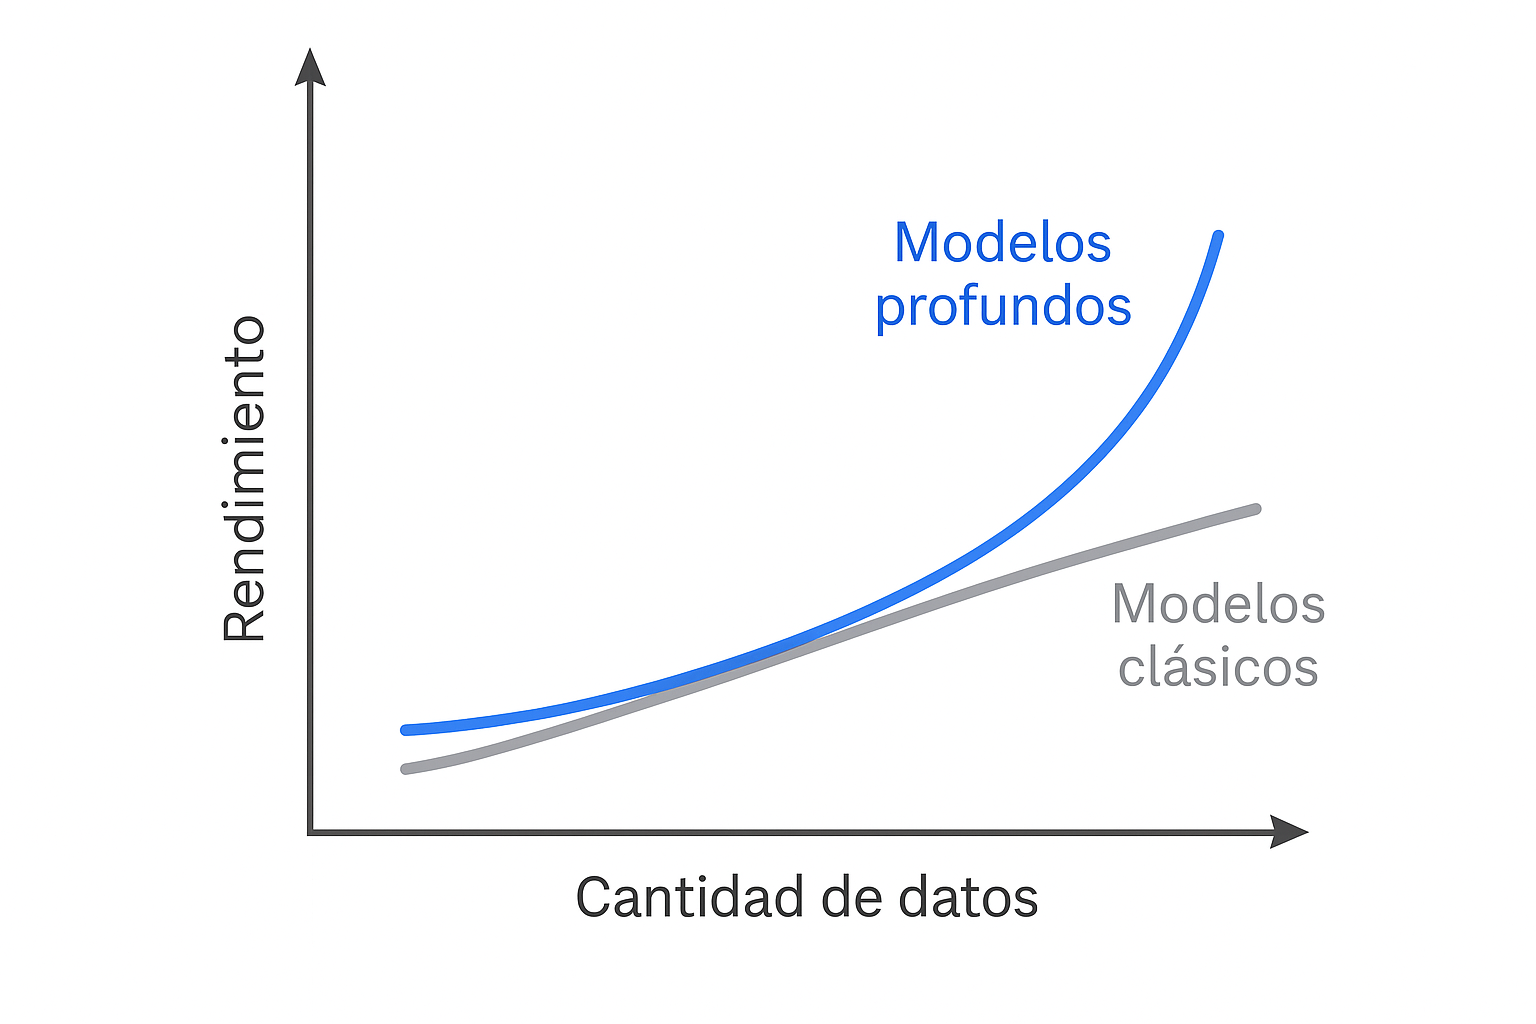
\includegraphics[width=.7\textwidth]{models-comp.png}
  \begin{block}{Regla empírica}
    Modelos profundos superan a los clásicos cuando los datos \(\uparrow\)
    y la complejidad del problema es alta.
  \end{block}
\end{frame}

% 8. Requisitos computacionales
\begin{frame}{Hardware y escalabilidad}
  \begin{itemize}
    \item Entrenamiento \(\sim\) GFlops–TFlops; inferencia en dispositivos móviles posible.
    \item GPUs y TPUs aceleran multiplicaciones matriz–vector.
    \item Distribución de datos y modelos: Data Parallel \& Model Parallel.
  \end{itemize}
  \begin{center}
    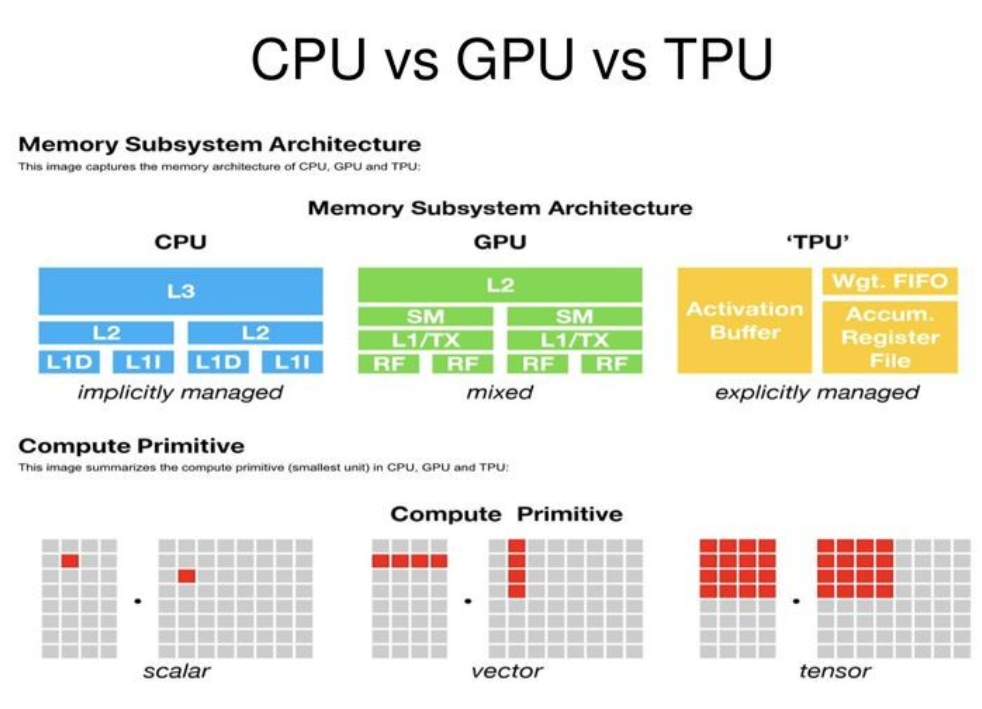
\includegraphics[width=.65\textwidth]{gpu-tpu.png}
  \end{center}
\end{frame}

% 9. Aplicaciones icónicas
\begin{frame}{Aplicaciones destacadas}
  \begin{columns}[T]
    \begin{column}{.48\textwidth}
      \textbf{IA (general)}
      \begin{itemize}
        \item Sistemas expertos médicos.
        \item Planificación automática en logística.
        \item Robótica industrial.
      \end{itemize}
      \vspace{.5em}
      \textbf{ML clásico}
      \begin{itemize}
        \item Créditos bancarios.
        \item Motores de recomendación básicos.
        \item Detección de fraude (reglas + SVM).
      \end{itemize}
    \end{column}
    \begin{column}{.48\textwidth}
      \textbf{Deep Learning}
      \begin{itemize}
        \item Reconocimiento de imágenes (ImageNet).
        \item Traducción automática (Transformers).
        \item Chatbots y LLMs (GPT-x).
      \end{itemize}
    \end{column}
  \end{columns}
\end{frame}

% 10. Cierre
\begin{frame}{Conclusiones}
  \begin{itemize}
    \item IA \(\supset\) ML \(\supset\) DL/DNN.
    \item DL domina cuando hay datos masivos y poder de cómputo.
    \item Algoritmos clásicos siguen siendo competitivos con pocos datos o
          requisitos de interpretabilidad altos.
  \end{itemize}
  \begin{block}{Enlaces sugeridos}
    \begin{itemize}
      \item Yann LeCun, “Deep Learning”, \url{http://yann.lecun.com/deep-learning/}
      \item MIT 6.S191, \url{https://introtodeeplearning.mit.edu}
    \end{itemize}
  \end{block}
\end{frame}



% ==========================================================
\section{Panorama general}
% ----------------------------------------------------------
\begin{frame}{Deep Learning en el contexto de la IA}
  \begin{itemize}
    \item \textbf{Inteligencia Artificial (IA):} Sistemas capaces de realizar tareas que normalmente requieren inteligencia humana.
    \item \textbf{Machine Learning (ML):} Sub--campo de IA que aprende patrones a partir de datos (\emph{programación basada en datos}).
    \item \textbf{Deep Learning (DL):} Sub--campo de ML que utiliza redes neuronales profundas para modelar funciones altamente no--lineales.
  \end{itemize}
  \begin{block}{Regla de oro}
    Mientras más datos, mejor se comporta el modelo \emph{(a diferencia de muchos algoritmos clásicos).}
  \end{block}
\end{frame}

\begin{frame}{Taxonomía rápida de ML}
  \begin{columns}[T]
    \begin{column}{0.5\textwidth}
      \textbf{Aprendizaje supervisado}
      \begin{itemize}
        \item Clasificación
        \item Regresión
        \item Ej.: filtro de spam, predicción de precios.
      \end{itemize}
      \vspace{1em}
      \textbf{Aprendizaje por refuerzo}
      \begin{itemize}
        \item Agente + entorno + recompensas.
        \item Ej.: AlphaGo, control de robots.
      \end{itemize}
    \end{column}
    \begin{column}{0.5\textwidth}
      \textbf{Aprendizaje no supervisado}
      \begin{itemize}
        \item Clustering (\emph{k}-means)
        \item Modelos generativos (GAN, autoencoders)
      \end{itemize}
      \vspace{1em}
      \textbf{Semi--supervisado / Auto--supervisado}
      \begin{itemize}
        \item Mezcla etiquetas + datos sin etiquetar.
      \end{itemize}
    \end{column}
  \end{columns}
\end{frame}

\begin{frame}[fragile]
\frametitle{Descomponiendo DL}
\begin{columns}
\begin{column}{0.4\textwidth}
\begin{itemize}\small
    \item En su forma b\'asica los modelos DL son dise\~nados usando redes neuronales.
    \item Una red es una organizaci\'on jer\'arquica de neuronas con conecci\'on a otras neuronas.
    \item Las neuronas pasan un mensaje o se\~nal a otras neuronas basadas en lo que reciben, y as\'i aprenden con alg\'un mecanismo de \textit{feedback}
    \item A la derecha hay una representaci\'on simplista de una red neuronal.
\end{itemize}
\end{column}
\begin{column}{0.6\textwidth}  %%<--- here
    \begin{center}
     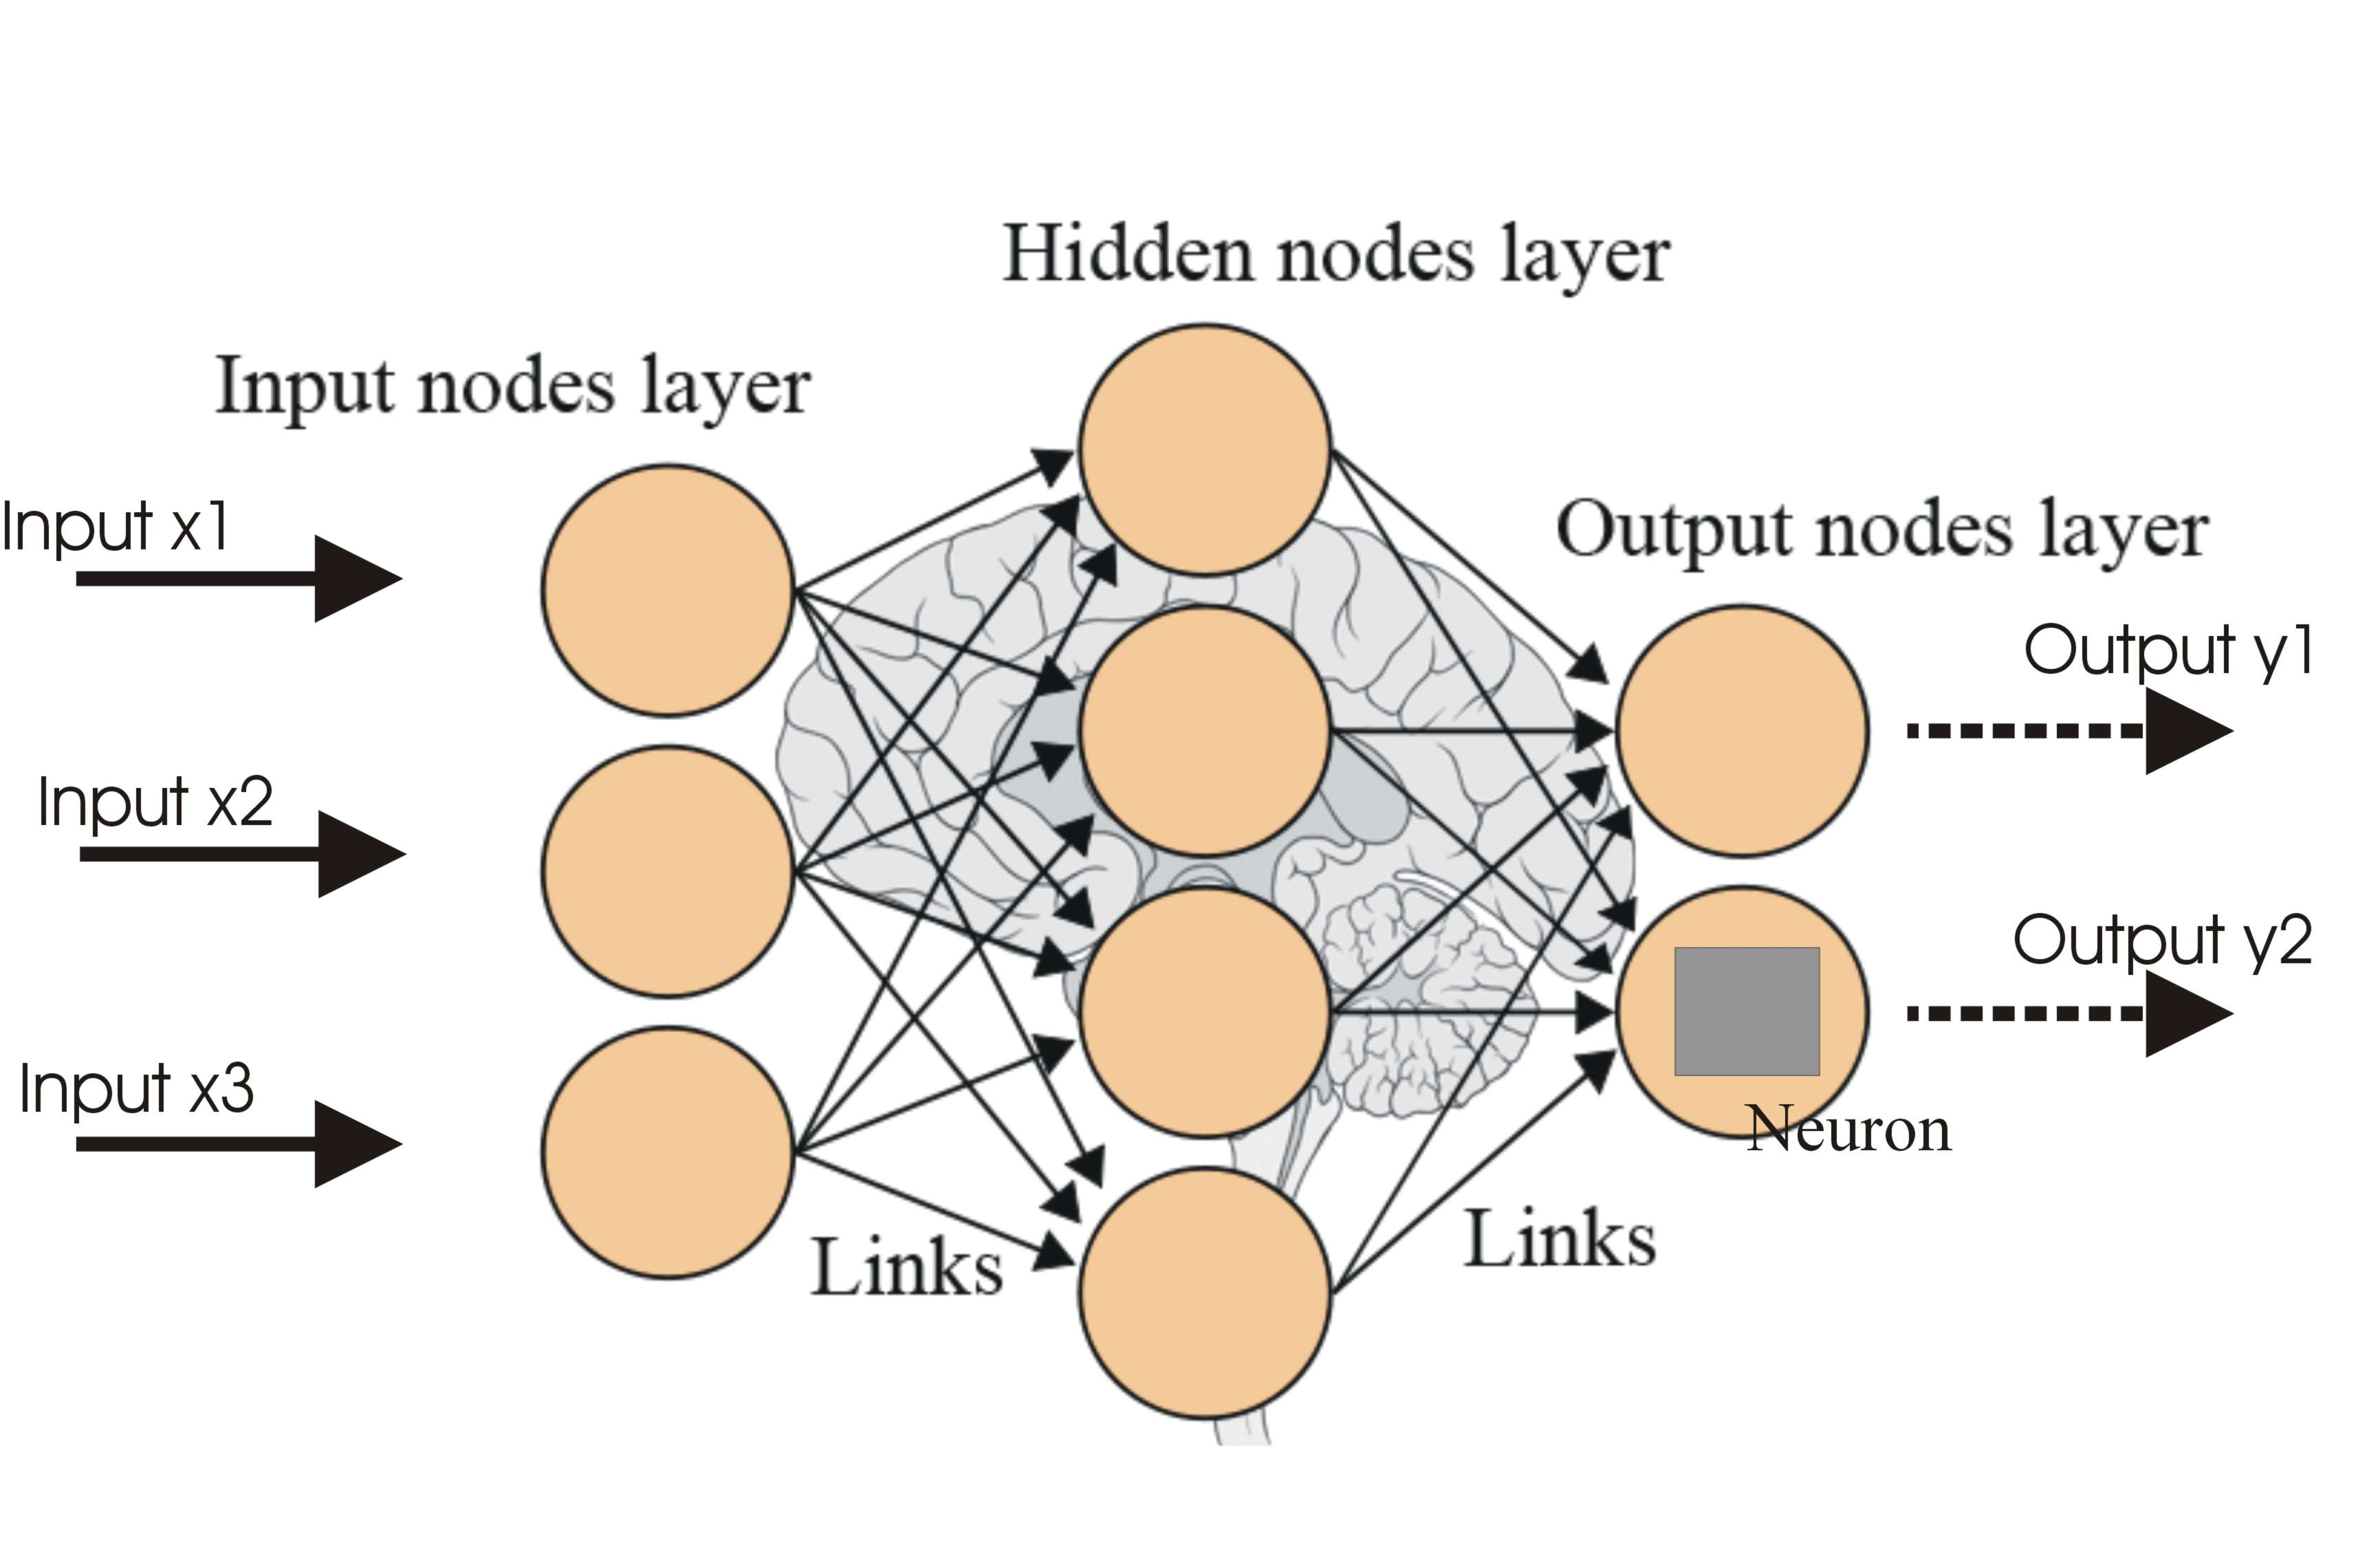
\includegraphics[width=1.0\textwidth]{simplenn.jpg}
     \end{center}
\end{column}
\end{columns}
\end{frame}


% ==========================================================
\section{Redes Neuronales}
% ----------------------------------------------------------
% ---------- BLOQUE 1 : La neurona artificial (5 slides) ---
\begin{frame}[fragile]{1/5  -  La neurona artificial: idea básica}
  \centering
  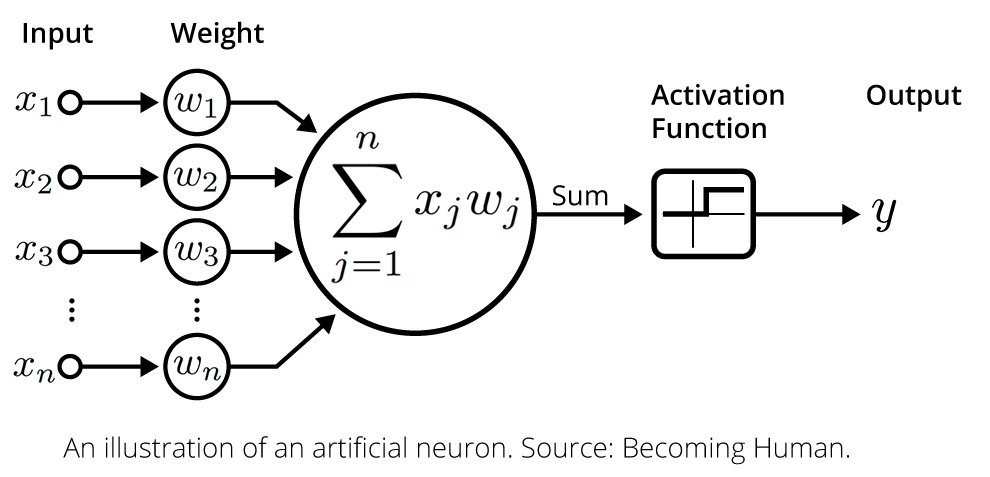
\includegraphics[width=.55\textwidth]{neurona.png}

  \[
    y = f\!\Big(\sum_{i=1}^{n} x_i\,\omega_i + b\Big)
  \]

  \begin{itemize}
    \item \textbf{Potencial}: suma ponderada + sesgo.
    \item \textbf{Activación \(f\)}: introduce no-linealidad.
    \item Con varias neuronas \(\rightarrow\) capa densa.
  \end{itemize}
\end{frame}

\begin{frame}[fragile]{2/5  -  Funciones de activación}
  \begin{columns}[T]
    \begin{column}{.48\textwidth}
      \begin{itemize}
        \item Sigmoide: $\sigma(z)=1/(1+e^{-z})$
        \item \textsc{tanh}: rango \([-1,1]\)
        \item \textbf{ReLU}: \(\max(0,z)\)
        \item ReLU6, Leaky-ReLU, GELU \ldots
      \end{itemize}
    \end{column}
    \begin{column}{.48\textwidth}
      \centering
      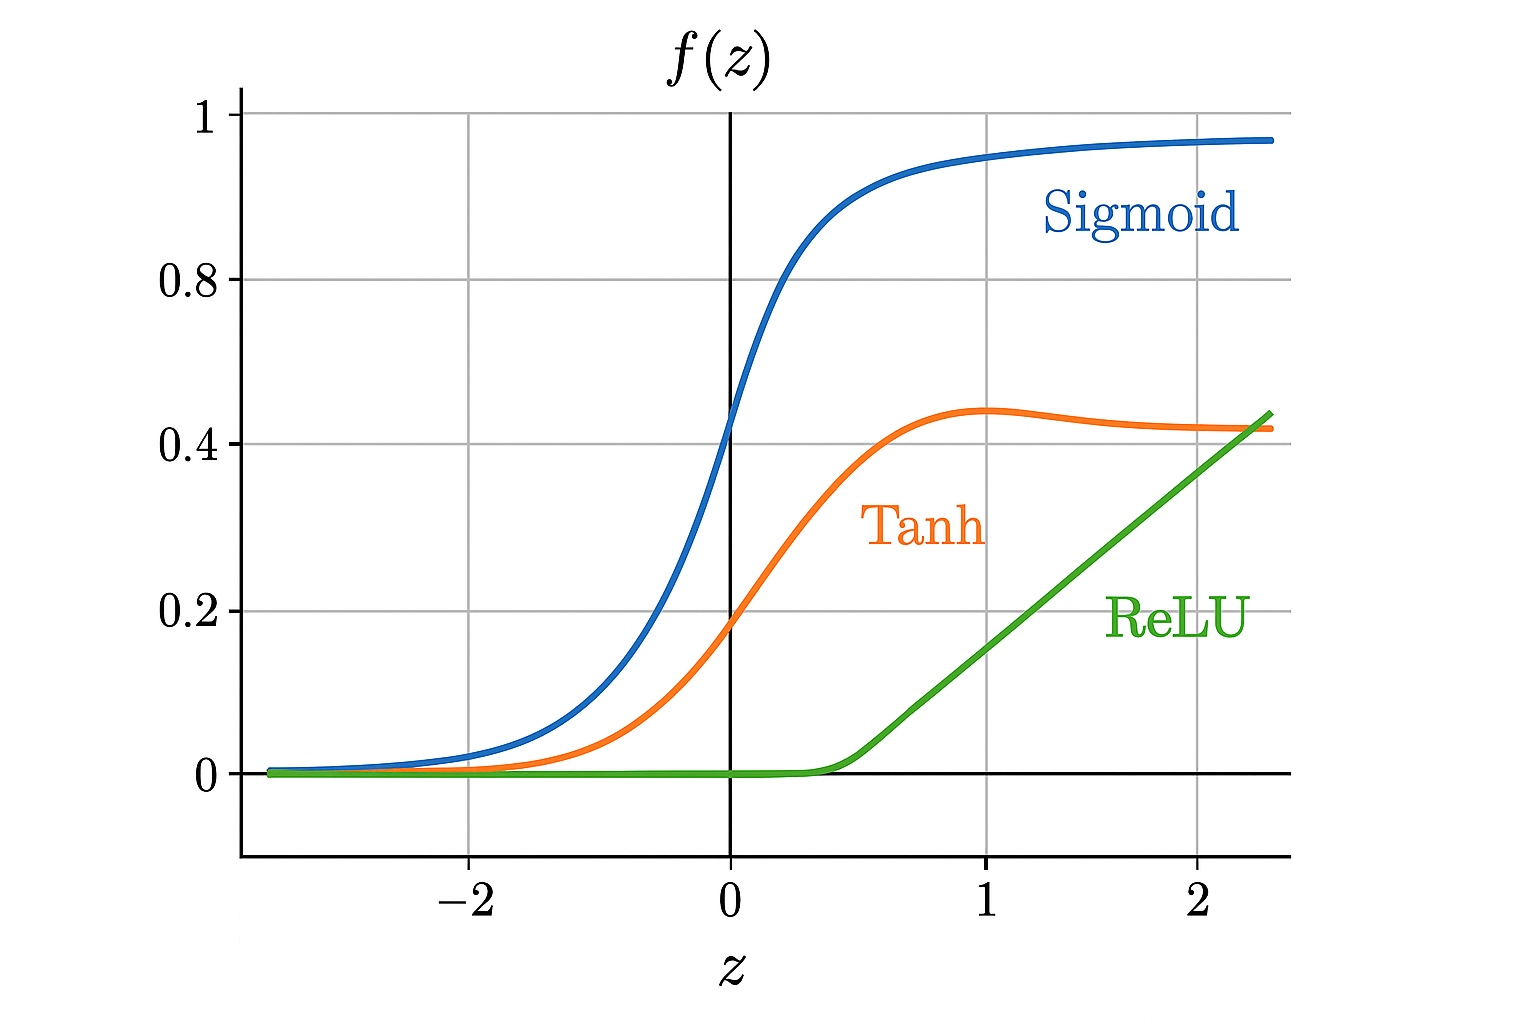
\includegraphics[width=\linewidth]{fun_activ.png}
    \end{column}
  \end{columns}
  \begin{block}{Tip}
    ReLU acelera el entrenamiento profundo y evita saturación de gradientes.
  \end{block}
\end{frame}

\begin{frame}[fragile]{3/5  -  Keras: construyendo una neurona}
  \begin{minted}[fontsize=\footnotesize]{python}
from tensorflow.keras import layers, Sequential

# x -> y = ReLU(Wx + b)
model = Sequential([
    layers.Dense(1, activation='relu',
                 input_shape=(n_features,))
])
y_pred = model(x_batch)
  \end{minted}
  \vspace{-1em}
  \begin{itemize}
    \item `Dense(1)` = 1 neurona.
    \item Parámetros aprendibles: \(n_\text{feat}+1\).
  \end{itemize}
\end{frame}

\begin{frame}{4/5  -  Vectorización y batch-processing}
  \begin{itemize}
    \item Entrenamos \(m\) ejemplos en paralelo:
      \(Y = f(XW + b)\)
    \item `X` \((m \times n)\) multiplica los pesos \((n \times 1)\).
    \item GPU = miles de neuronas / ejemplos simultáneos.
  \end{itemize}
  \centering
  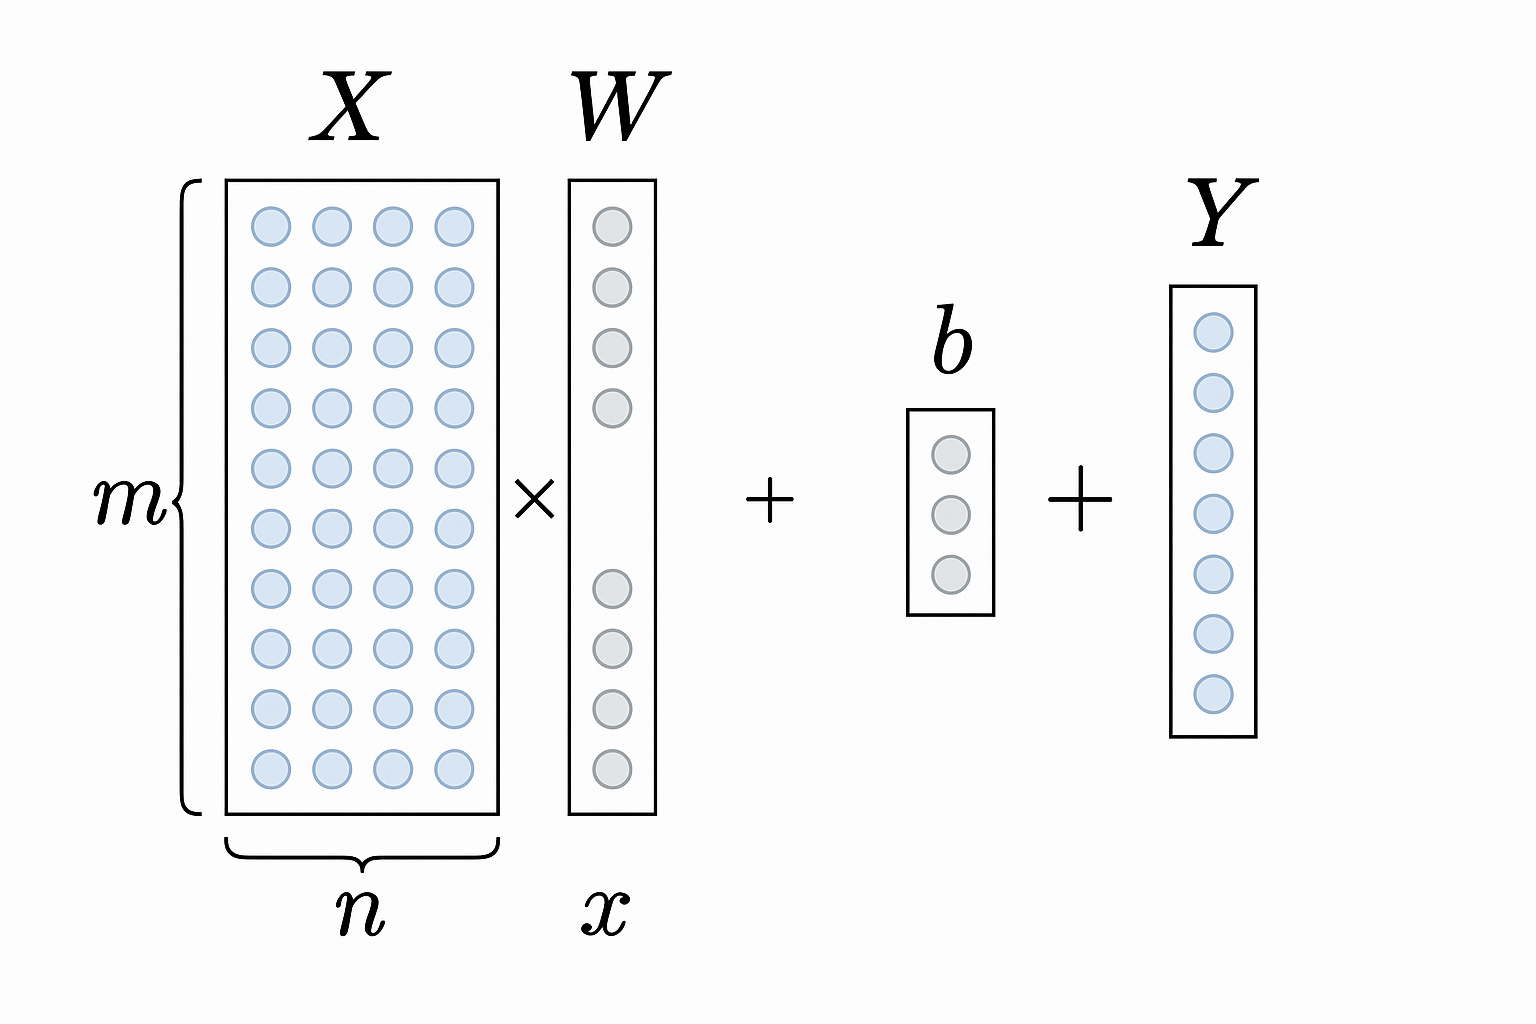
\includegraphics[width=.6\textwidth]{vectoriz.png}
\end{frame}

\begin{frame}{5/5  -  Capas densas encadenadas}
  \begin{itemize}
    \item Salida de una capa = entrada de la siguiente.
    \item Cada capa aprende representaciones de mayor nivel.
    \item Profundidad \(\uparrow\) \(\Rightarrow\) capacidad \(\uparrow\),
          riesgo de sobreajuste \(\uparrow\).
  \end{itemize}
  \centering
  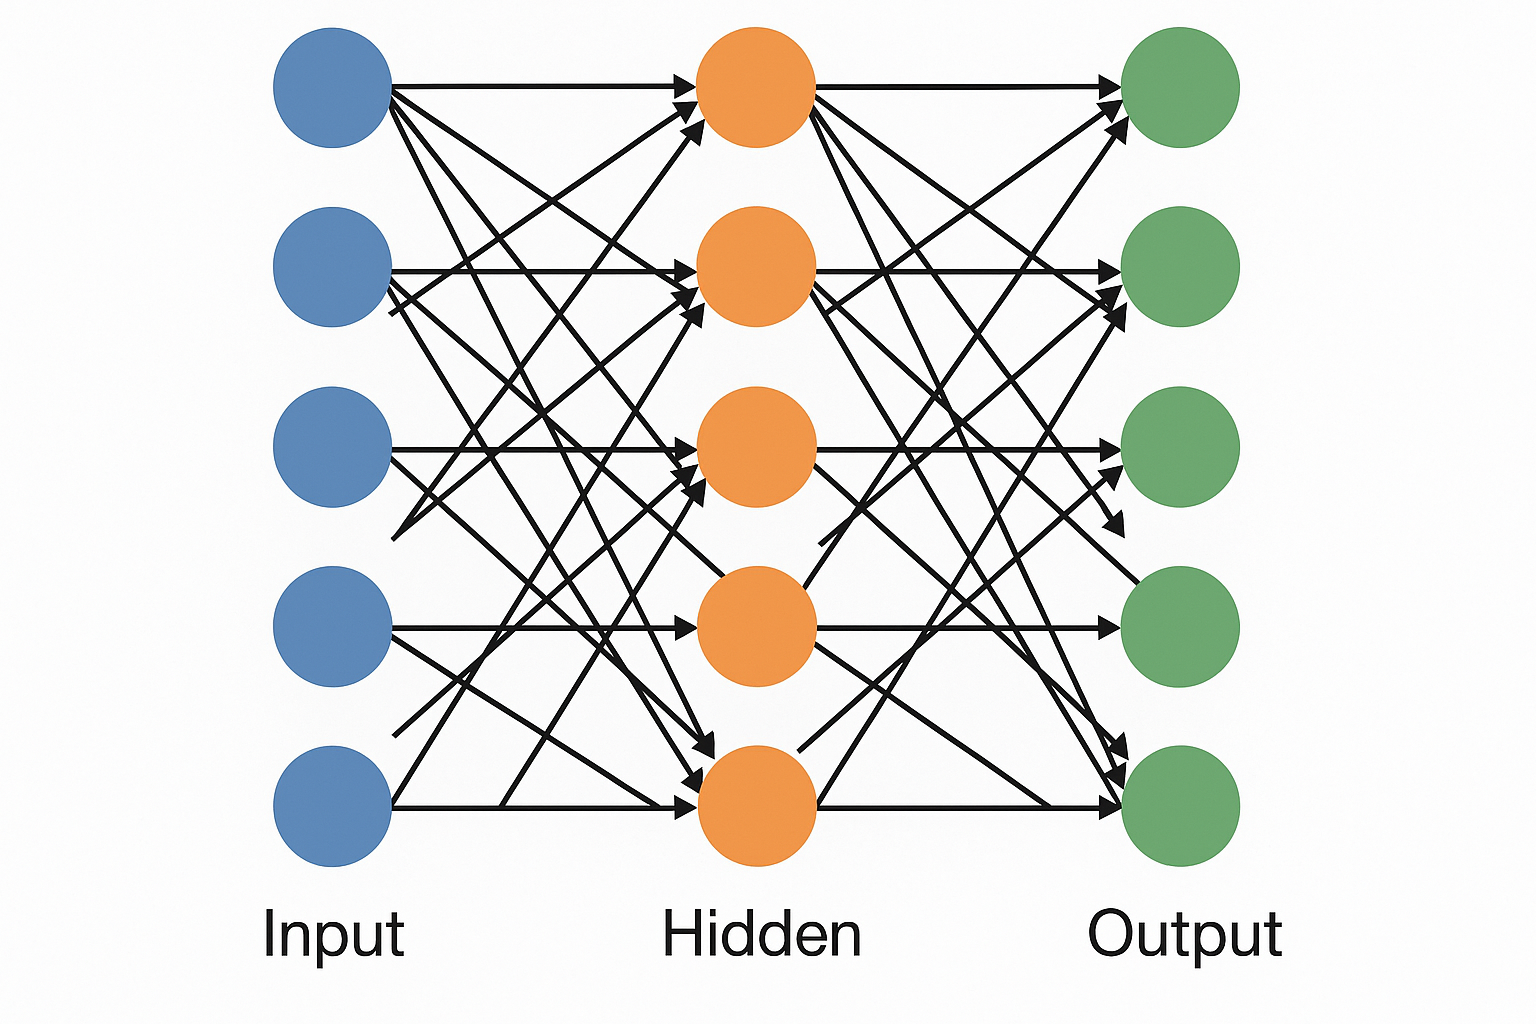
\includegraphics[width=.55\textwidth]{inp-hid-out.png}
\end{frame}

% ---------- TRANSICIÓN : de capas densas a arquitecturas clásicas ----------
\begin{frame}[fragile]{De capas densas encadenadas a MLPs}
  \begin{center}
    \large\bfseries
    De la \emph{idea} de encadenar capas\\[0.3em]
    a la \emph{arquitectura} Perceptrón Multicapa
  \end{center}
  \vspace{0.2cm}

  \begin{itemize}
    \item Una red de \textbf{capas densas encadenadas} (\emph{feed--forward}) ya es capaz de aproximar funciones complejas, pero sigue siendo \alert{lineal} si no aplicamos activaciones.

    \item Al intercalar \textbf{activaciones no lineales} (ReLU, tanh, GELU, etc.) cada capa aprende representaciones más abstractas. \\[0.6em]

    \item El siguiente paso natural es el \textbf{Perceptrón Multicapa (MLP)}, que extiende esta idea a varias capas ocultas y se convierte en un \emph{aproximador universal}.

    \item A continuación exploraremos \emph{arquitecturas clásicas}: MLP, CNN, RNN, etc.
  \end{itemize}

  \begin{center}
    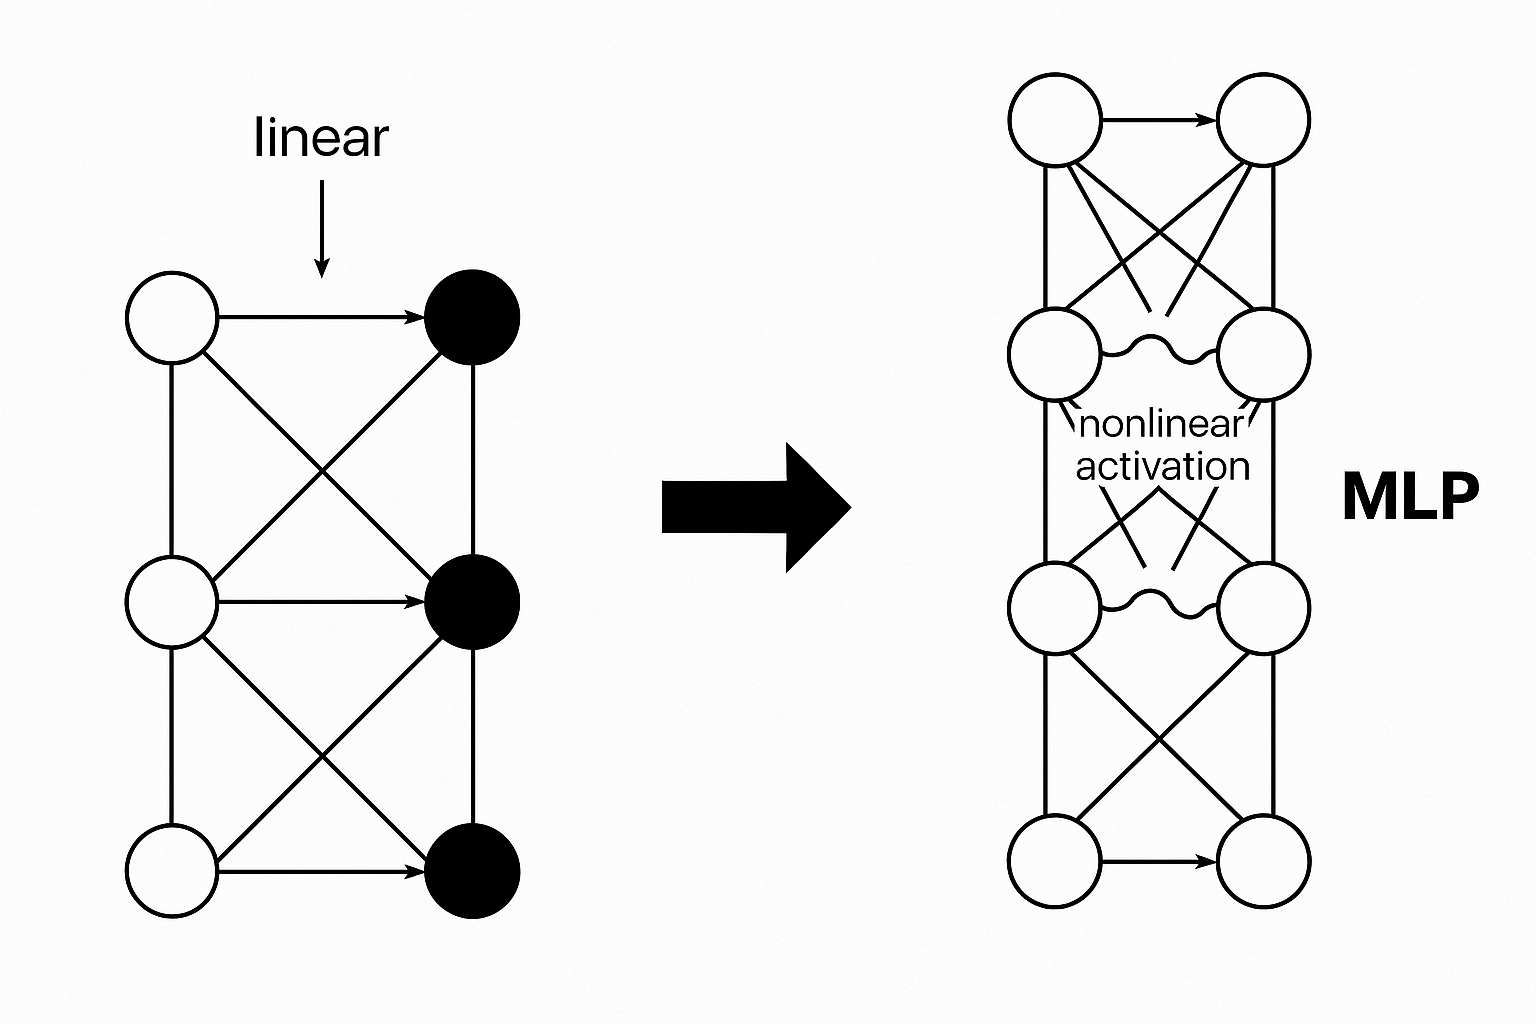
\includegraphics[width=.52\textwidth]{dense_To_mlp.png}
  \end{center}
\end{frame}



% ---------- BLOQUE 2 : Arquitecturas clásicas (5 slides) ---
\begin{frame}[fragile]{1/5  -  Perceptrón multicapa (MLP)}
  \begin{itemize}
    \item Capas densas + activaciones no-lineales.
    \item Adecuado para datos tabulares o embeddings.
  \end{itemize}
  \begin{minted}[fontsize=\footnotesize]{python}
model = Sequential([
    layers.Dense(128, activation='relu', input_shape=(784,)),
    layers.Dense(64, activation='relu'),
    layers.Dense(10, activation='softmax')
])
  \end{minted}
  \centering
  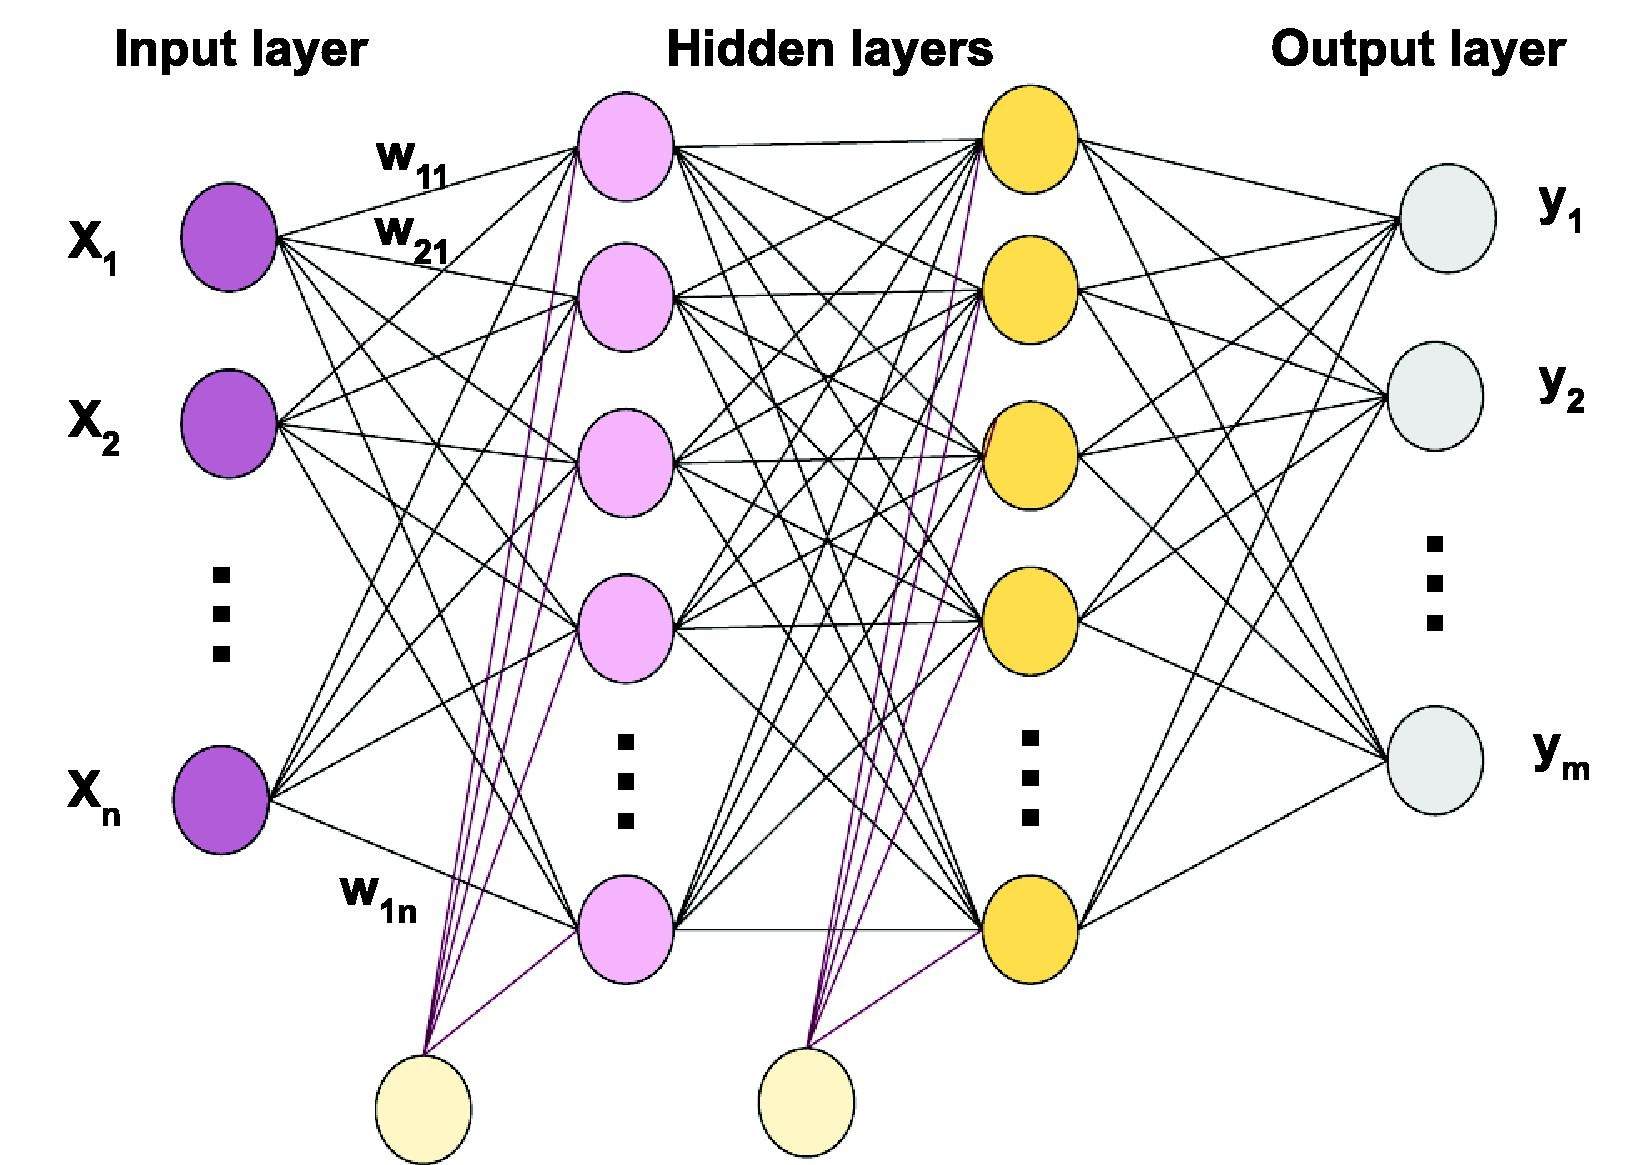
\includegraphics[width=.5\textwidth]{mlp_ex.jpg}\footnote{https://doi.org/10.1016/j.neucom.2023.126327}
\end{frame}

\begin{frame}[fragile]{2/5  -  Convolutional Neural Networks (CNN)}
  \begin{itemize}
    \item Filtros que comparten pesos \(\rightarrow\) detección local.
    \item Pooling reduce dimensionalidad y traslación.
  \end{itemize}
  \begin{minted}[fontsize=\footnotesize]{python}
model = Sequential([
  layers.Conv2D(32, 3, activation='relu',
                input_shape=(32,32,3)),
  layers.MaxPooling2D(2),
  layers.Conv2D(64, 3, activation='relu'),
  layers.Flatten(),
  layers.Dense(10, activation='softmax')
])
  \end{minted}
  \begin{center}
    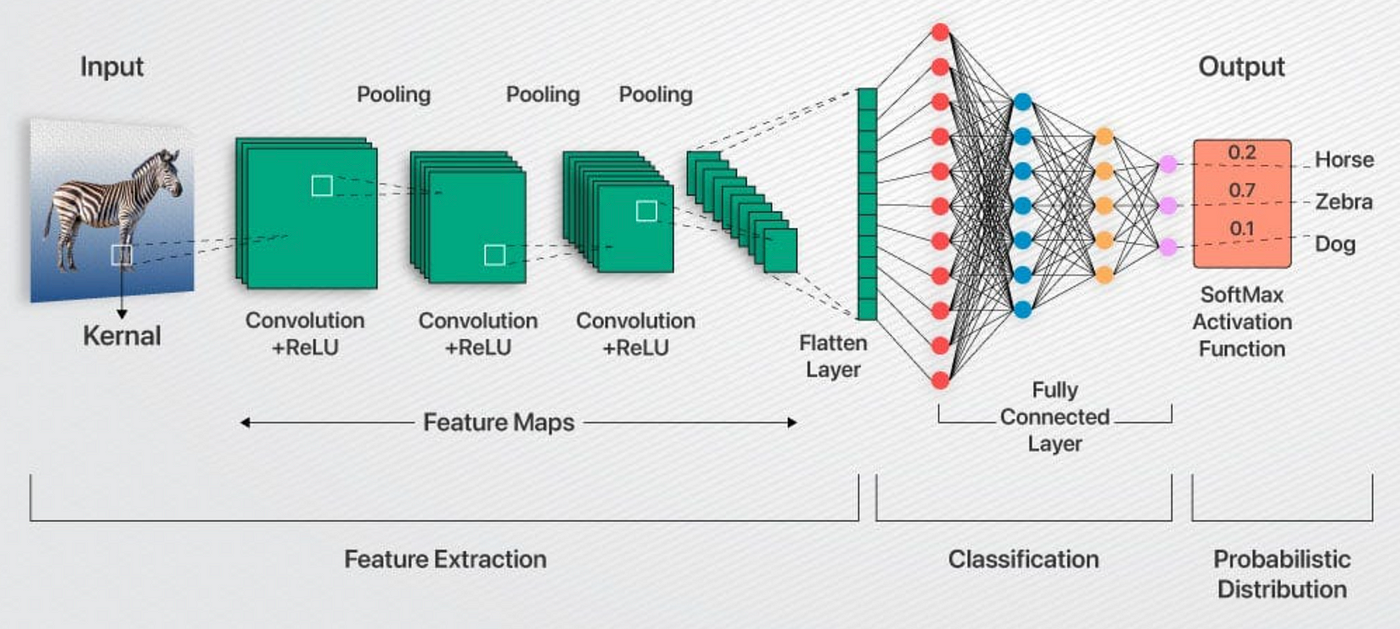
\includegraphics[width=.7\textwidth]{cnn_ex.png}
  \end{center}
\end{frame}

\begin{frame}[fragile]{3/5  -  Redes recurrentes (RNN, LSTM, GRU)}
  \begin{itemize}
    \item Estado interno \(h_t\) que se recicla en el tiempo.
    \item Modela secuencias: texto, audio, series temporales.
  \end{itemize}
  \begin{minted}[fontsize=\footnotesize]{python}
model = Sequential([
    layers.Embedding(vocab, 128),
    layers.LSTM(64),
    layers.Dense(1, activation='sigmoid')
])
  \end{minted}
  \begin{center}
    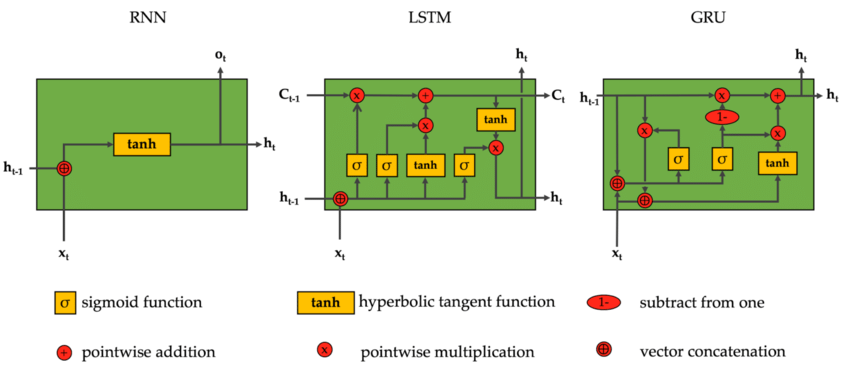
\includegraphics[width=.75\textwidth]{rnn-lstm-gru_ex.png}
  \end{center}
\end{frame}

\begin{frame}[fragile]{4/5  -  Autoencoders}
  \begin{itemize}
    \item Codificador \(x \rightarrow z\); decodificador \(z \rightarrow \hat{x}\).
    \item Objetivo: reconstruir entrada \(\Rightarrow\) compresión no lineal.
    \item Base de denoising, GAN, VAEs.
  \end{itemize}
  \begin{minted}[fontsize=\footnotesize]{python}
encoded = layers.Dense(32, activation='relu')(inputs)
decoded = layers.Dense(784, activation='sigmoid')(encoded)
autoencoder = keras.Model(inputs, decoded)
  \end{minted}
  \begin{center}
    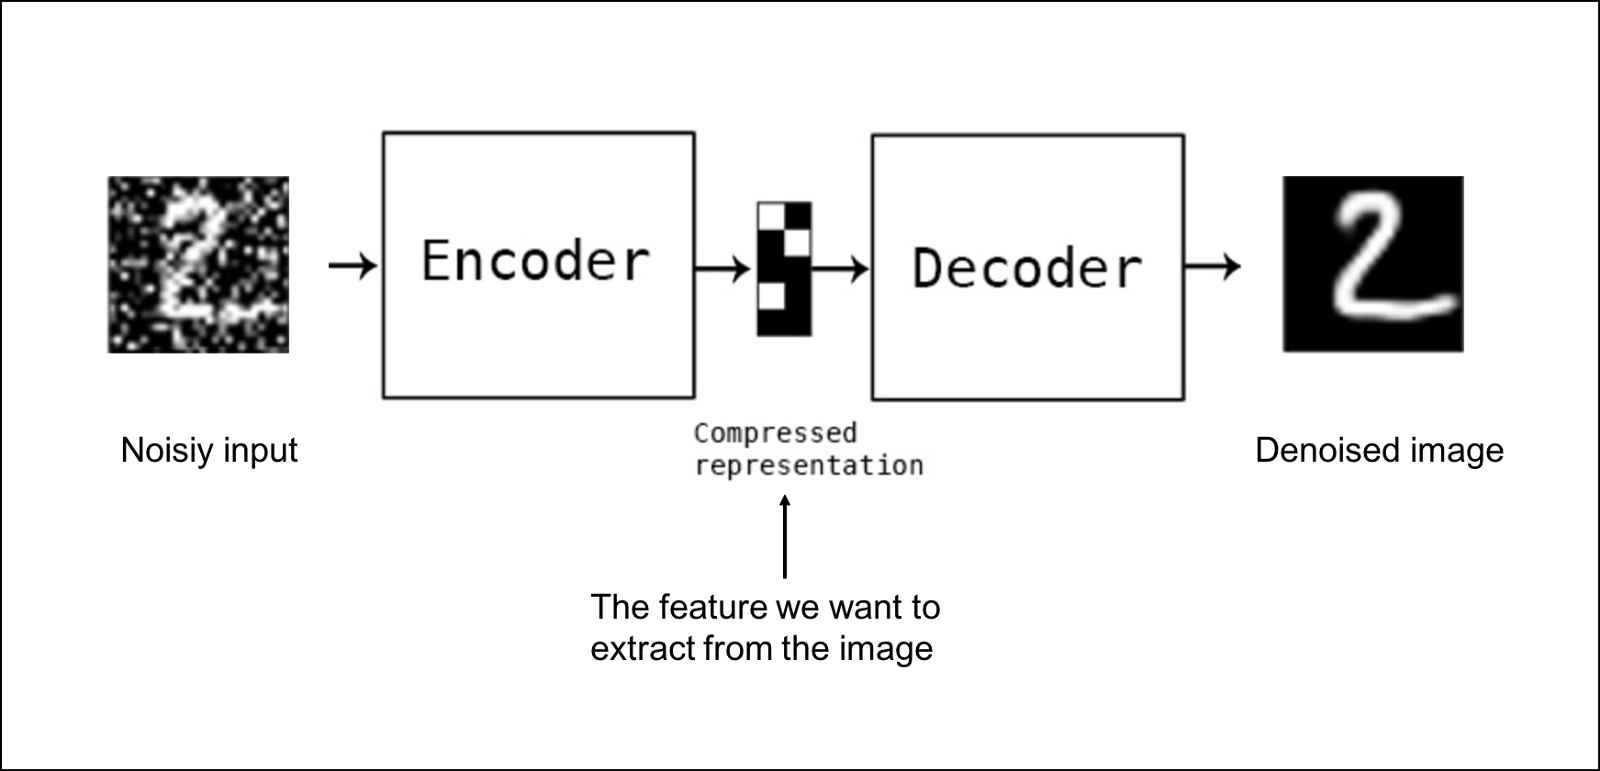
\includegraphics[width=.75\textwidth]{a1.png}
  \end{center}
\end{frame}

\begin{frame}{5/5  -  Transformers (bonus)}
  \begin{itemize}
    \item Mecanismo de \textbf{atención}: pesos dinámicos por token.
    \item Paraleliza secuencias mejor que RNN.
    \item BERT, GPT-x, Vision-Transformer.
  \end{itemize}
  \centering
  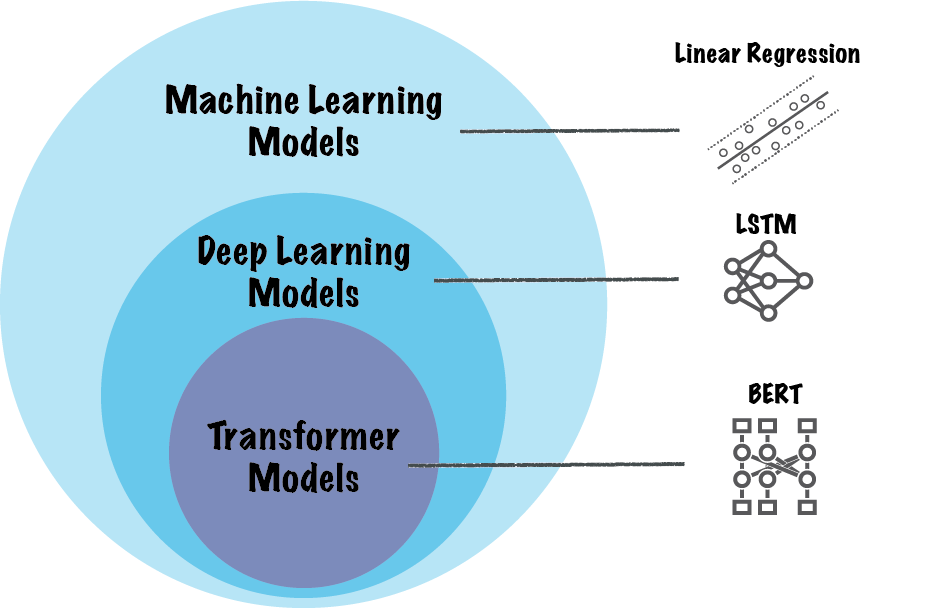
\includegraphics[width=.6\textwidth]{ml_models-transf.png}
\end{frame}

% ---------- BLOQUE 3 : Forward y Back-propagation (5 slides) ---
\begin{frame}[fragile]{1/5  -  Pipeline de entrenamiento}
  \begin{center}
    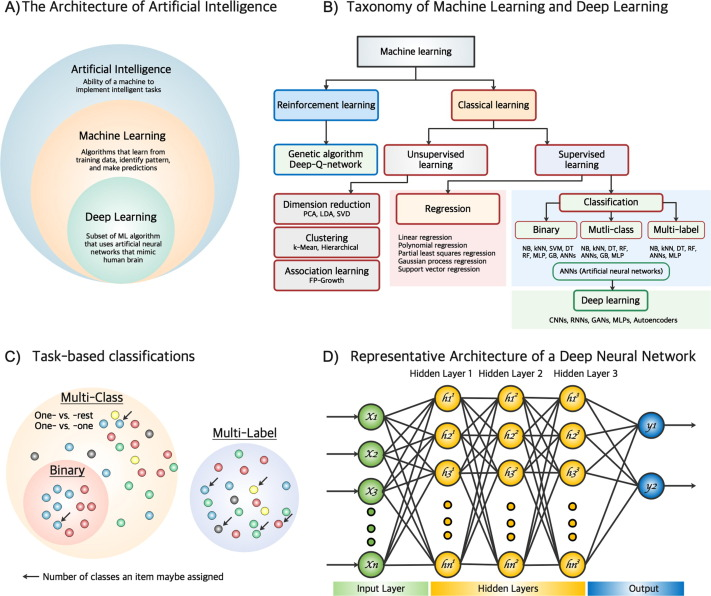
\includegraphics[width=0.6\textwidth]{Pipeline-training.jpg}
  \end{center}
  \begin{enumerate}
    \item Forward pass: \(x \rightarrow y_{pred}\)
    \item Cálculo de pérdida \(J\)
    \item Back-prop: gradientes \(\nabla_{\!\omega}J\)
    \item Actualización de pesos
  \end{enumerate}
\end{frame}

%------------------------------------------------------------------
% 2/5 – Funciones de pérdida habituales
%------------------------------------------------------------------
\begin{frame}[fragile]{2/5  --  Funciones de pérdida habituales}
  \begin{columns}[T]
    %-------------------------------- LEFT COLUMN
    \begin{column}[T]{0.55\textwidth}\small
      \begin{block}{Clasificación multiclase}
        \[
          \mathcal{L}_{\text{CE}}
            = -\sum_{k=1}^{C} y_k \,\log \hat y_k
        \]
        \footnotesize
        (Sólo usa la fila verdadera del vector one--hot,
        se implementa como \verb|CategoricalCrossentropy|).
      \end{block}

      \begin{block}{Regresión}
        \[
          \mathcal{L}_{\text{MSE}}
            = \frac{1}{N}\sum_{i=1}^{N}
              \left(y_i - \hat y_i\right)^{2}
        \]
        \footnotesize
        Penaliza errores grandes de forma cuadrática.
      \end{block}

      \begin{block}{Autoencoder variacional (VAE)}
        \[
          \mathcal{L}_{\text{ELBO}}
            = \underbrace{\mathbb{E}_{q_\phi(z|x)}
                [-\log p_\theta(x|z)]}_{\text{reconstrucción}}
              \;+\;
              \underbrace{\text{KL}\!
                \bigl(q_\phi(z|x)\;\|\;p(z)\bigr)}_{\text{regularización}}
        \]
        \footnotesize
        Equilibra fidelidad y regularización bayesiana.
      \end{block}
    \end{column}

    %-------------------------------- RIGHT COLUMN
    \begin{column}[T]{0.45\textwidth}
      % parbox :  altura = 90 % de la altura útil de la diapositiva
      \parbox[c][0.9\textheight][c]{\linewidth}{%
        \centering
        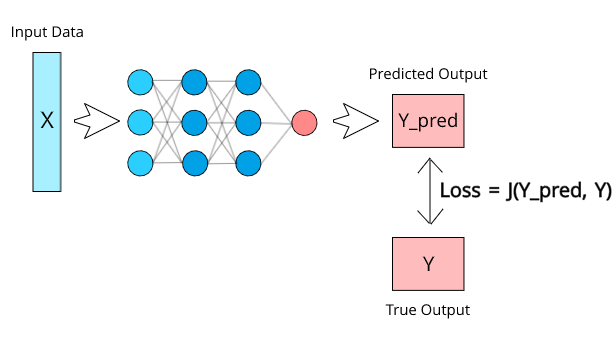
\includegraphics[width=.9\linewidth]{loss_func.png}\par
        \vspace{0.4em}
        \scriptsize\color{gray}{\emph{Función de pérdida.}}%
      }
    \end{column}
  \end{columns}
\end{frame}

%------------------------------------------------------------------
% 3/5 – Algoritmos de optimización
%------------------------------------------------------------------
\begin{frame}[fragile]{3/5  --  Algoritmos de optimización}
  \begin{columns}[T]
    %-------------------------------- LEFT COLUMN
    \begin{column}{0.52\textwidth}
      \textbf{Descenso de gradiente estocástico (SGD)}
      \[
        \theta_{t+1}
          = \theta_t \;-\;
            \eta\,\nabla_\theta
            \mathcal{L}\bigl(\theta_t; \mathcal{B}_t\bigr)
      \]
      \begin{itemize}
        \item Ligero, sin memoria extra.
        \item Ruido $\;\Rightarrow\;$ ayuda a escapar de mínimos locales.
        \item Sensible a la elección de \(\eta\) y al \emph{schedule}.
      \end{itemize}
    \end{column}

    %-------------------------------- RIGHT COLUMN
    \begin{column}{0.48\textwidth}
      \textbf{Adam (Adaptive Moment Estimation)}
      \[
        \begin{aligned}
          m_t &= \beta_1 m_{t-1} + (1-\beta_1) g_t \\\\
          v_t &= \beta_2 v_{t-1} + (1-\beta_2) g_t^{2} \\\\
          \hat m_t &= m_t /(1-\beta_1^{t}) \\\\
          \hat v_t &= v_t /(1-\beta_2^{t}) \\\\
          \theta_{t+1} &= \theta_t - \eta\,\hat m_t/\bigl(\sqrt{\hat v_t}+\varepsilon\bigr)
        \end{aligned}
      \]
      \begin{itemize}
        \item Paso adaptativo por parámetro.
        \item Converge rápido, estable en datos dispersos.
        \item Más memoria (\(2\times\) parámetros) $\;\&\;$ requiere
              \(\beta_{1,2}\) y \(\varepsilon\).
      \end{itemize}
    \end{column}
  \end{columns}

  \vspace{0.35em}
  \hrule
  \vspace{0.35em}

  \centering
  \small
  Otros optimizadores: \textbf{RMSProp}, \textbf{Adagrad},
  \textbf{AdamW} (decay), \textbf{Nadam} (momentum de Nesterov)\,…
\end{frame}


\begin{frame}[fragile]{4/5  -  Entrenamiento en Keras}
  \begin{minted}[fontsize=\footnotesize]{python}
model.compile(optimizer='adam',
              loss='sparse_categorical_crossentropy',
              metrics=['accuracy'])
history = model.fit(train_ds,
                    epochs=20,
                    validation_data=val_ds)
  \end{minted}
  \begin{itemize}
    \item `compile` asocia pérdida y optimizador.
    \item `fit` maneja forward, back-prop y logging.
  \end{itemize}
\end{frame}

\begin{frame}{5/5  -  Buenas prácticas}
  \begin{itemize}
    \item \textbf{Normalizar} datos de entrada.
    \item \textbf{Early-stopping} para evitar sobreajuste.
    \item Dropout y regularización L2.
    \item Learning rate schedule / warm-up.
  \end{itemize}
  \centering
  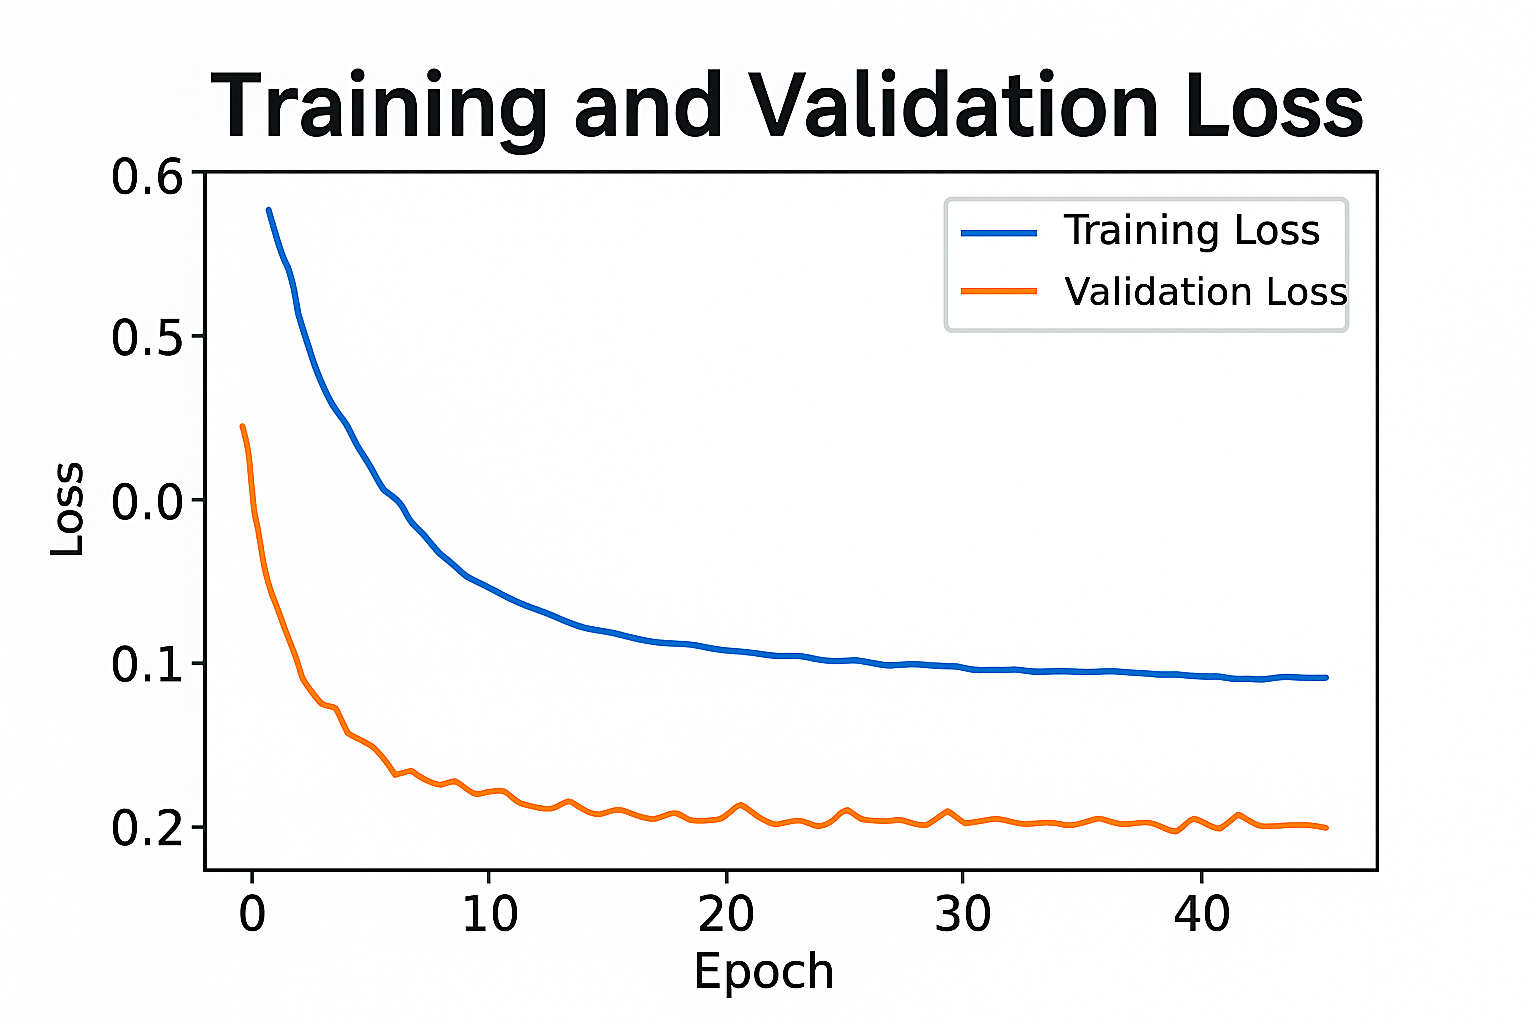
\includegraphics[width=.55\textwidth]{val_loss.png}
\end{frame}



\begin{comment}
% ==========================================================
\section{Redes Neuronales}
% ----------------------------------------------------------
\begin{frame}{La neurona artificial}
  \begin{equation*}
    y = f\!\big(\underbrace{\sum_{i=1}^{n} x_i\,\omega_i + b}_{\text{potencial}}\big)
  \end{equation*}
  \begin{itemize}
    \item $f$ \textbf{no--lineal}: Sigmoide, \textsc{tanh}, ReLU \ldots
    \item $\omega_i$ pesos; $b$ sesgo.
  \end{itemize}
  \begin{figure}[h]
    \centering
    \includegraphics[width=.6\linewidth]{example-image}
    \caption{Esquema de neurona y sus pesos.}
  \end{figure}
\end{frame}

\begin{frame}{Arquitecturas clásicas}
  \begin{itemize}
    \item \textbf{Perceptrón multicapa (MLP)}: Capas completamente conectadas.
    \item \textbf{Convolutional NN (CNN)}: Visión por computadora.
    \item \textbf{Recurrente (RNN / LSTM / GRU)}: Secuencias y series de tiempo.
    \item \textbf{Autoencoders}: Compresión, reducción de dimensión y generación.
  \end{itemize}
  \begin{figure}
    \centering
    \includegraphics[width=.8\linewidth]{example-image}
    \caption{Comparación de arquitecturas.}
  \end{figure}
\end{frame}

\begin{frame}{Forward y Back--propagation}
  \begin{itemize}
    \item \textbf{Forward}: Propaga la entrada hasta la salida.
    \item \textbf{Función de pérdida}: Qué tan lejos de la verdad.
    \item \textbf{Back--propagation}: Regla de la cadena para actualizar pesos.
  \end{itemize}
  \begin{equation*}
    \omega \leftarrow \omega - \eta\,\nabla_{\!\omega}J(\omega)
  \end{equation*}
  \pause
  \textit{SGD, Adam, RMSProp, \ldots}
\end{frame}
\end{comment}

% ==========================================================
\section{CNN en detalle}
% ----------------------------------------------------------
\begin{frame}{Convolutional Neural Networks (CNN)}
  \begin{itemize}
    \item Filtrado local y \textbf{parámetros compartidos}.  
    \item Stride, padding \& pooling para controlar dimensionalidad.
    \item Eficientes y con inductive bias para datos con estructura 2D/3D.
  \end{itemize}
  \begin{figure}
    \centering
    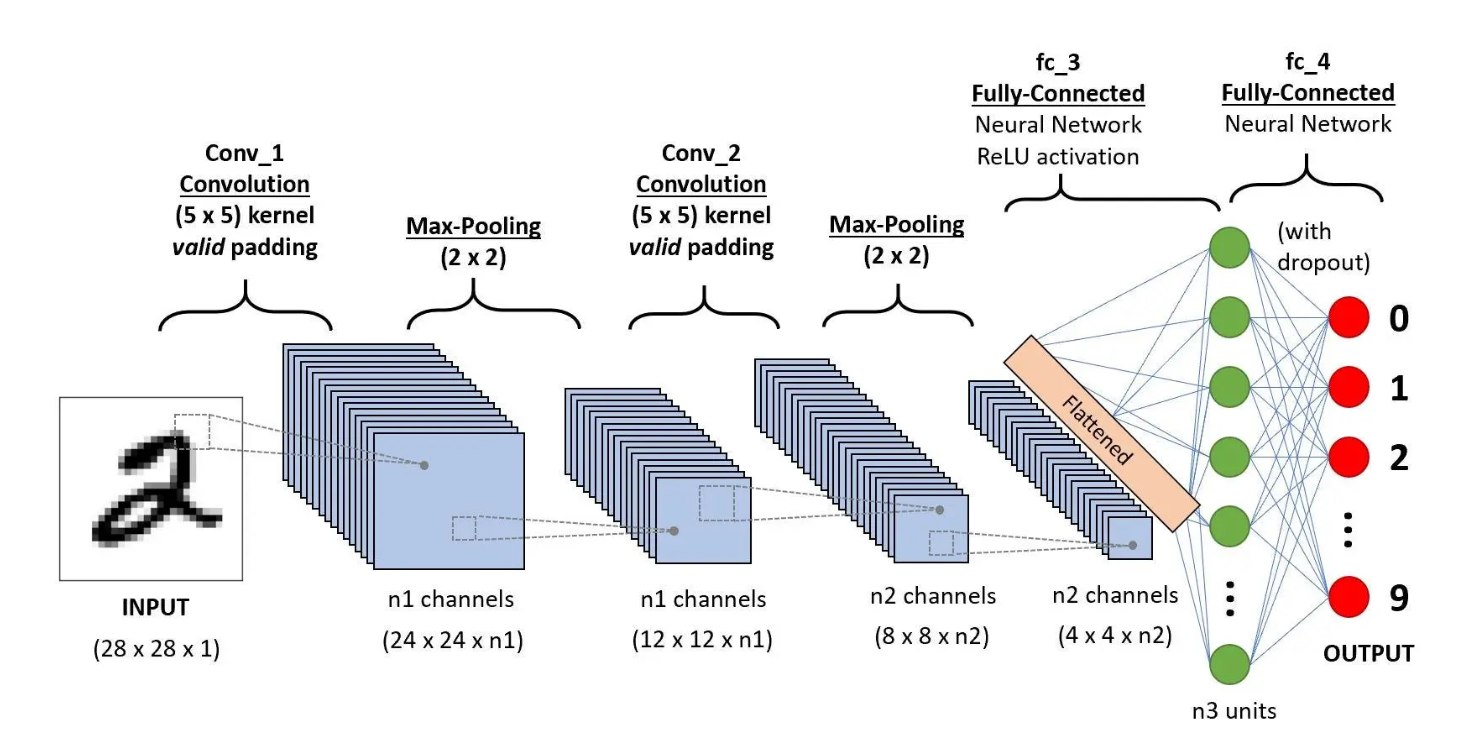
\includegraphics[width=.75\linewidth]{cnn.png}
    \caption{Proceso standard en CNN}
  \end{figure}
\end{frame}

\begin{frame}{Pooling y arquitectura típica}
  \begin{itemize}
    \item Max / Average pooling: reduce resolución, gana invariancia.
    \item Patrón frecuente: [Conv $\rightarrow$ ReLU]$^{\times n}$ $\rightarrow$ Pool.
  \end{itemize}
  \begin{figure}
    \centering
    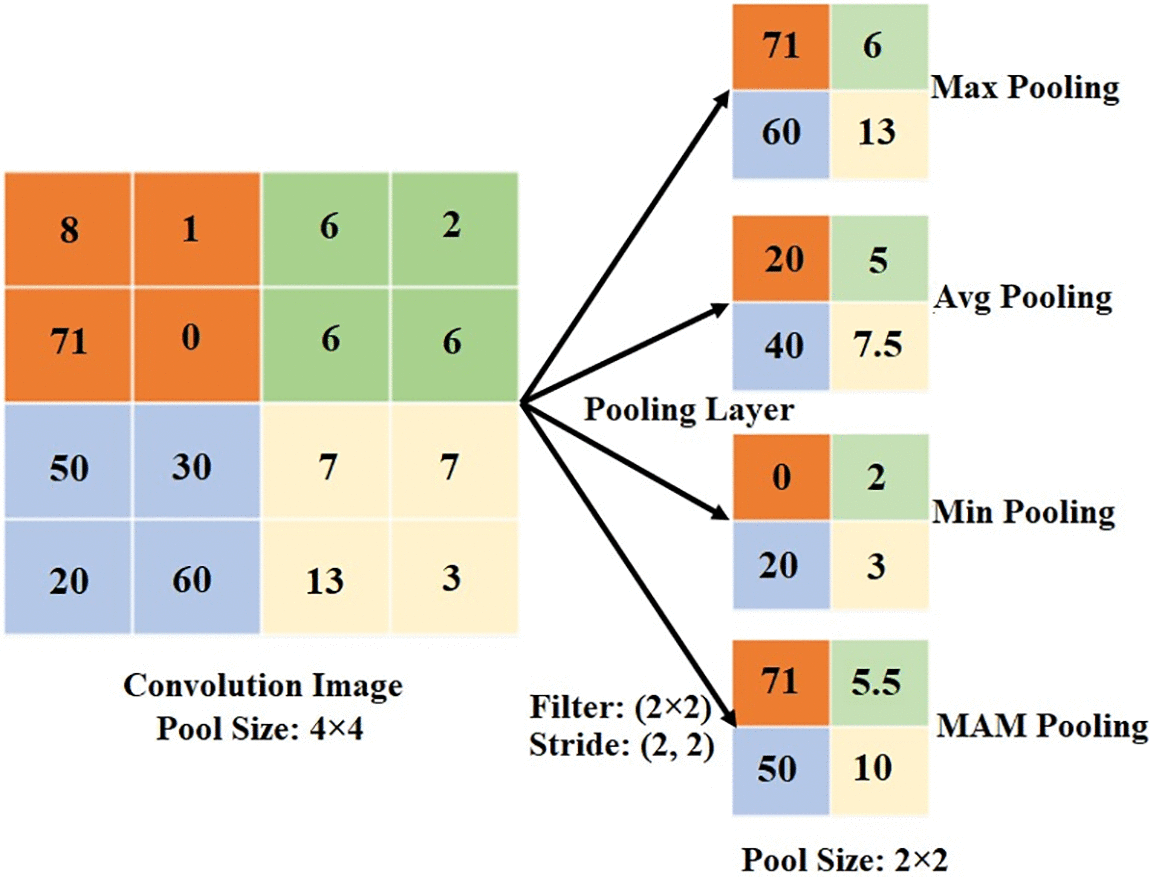
\includegraphics[width=.7\linewidth]{maxpool.png}
    \caption{Cadena Conv–Pool antes de Fully Connected.}
  \end{figure}
\end{frame}

% ==========================================================
\section{Regularización y Mejora de modelos}
% ----------------------------------------------------------
\begin{frame}{Estrategias de regularización}
  \begin{columns}
    \begin{column}{0.5\textwidth}
      \begin{itemize}
        \item Dropout
        \item Weight decay ($L_2$)
        \item Data augmentation
      \end{itemize}
    \end{column}
    \begin{column}{0.5\textwidth}
      \begin{itemize}
        \item Batch Normalization
        \item Early Stopping
        \item Transfer Learning
      \end{itemize}
    \end{column}
  \end{columns}
\end{frame}

% ==========================================================
\section{Ejemplos en Keras}
% ----------------------------------------------------------
\begin{frame}[fragile]{MLP mínimo en Keras}
  \begin{minted}[fontsize=\scriptsize]{python}
from keras.models import Sequential
from keras.layers import Dense
import numpy as np

x_train = np.random.random((6000, 10))
y_train = np.random.randint(2, size=(6000, 1))

model = Sequential([
    Dense(32, activation='relu', input_shape=(10,)),
    Dense(1, activation='sigmoid')
])
model.compile(optimizer='adam',
              loss='binary_crossentropy',
              metrics=['accuracy'])
model.fit(x_train, y_train, epochs=10, batch_size=64)
  \end{minted}
\end{frame}

\begin{frame}[fragile]{CNN para MNIST en 15 líneas}
  \begin{minted}[fontsize=\scriptsize]{python}
from keras.datasets import mnist
from keras.utils import to_categorical
from keras.models import Sequential
from keras.layers import Conv2D, MaxPool2D, Flatten, Dense

(X_train, y_train), (X_test, y_test) = mnist.load_data()
X_train = X_train.reshape(-1,28,28,1)/255.
X_test  = X_test.reshape(-1,28,28,1)/255.
y_train = to_categorical(y_train,10)
y_test  = to_categorical(y_test,10)

model = Sequential([
    Conv2D(32,(3,3),activation='relu',input_shape=(28,28,1)),
    MaxPool2D(),
    Flatten(),
    Dense(128,activation='relu'),
    Dense(10,activation='softmax')])
model.compile(optimizer='adam',
              loss='categorical_crossentropy',
              metrics=['accuracy'])
model.fit(X_train,y_train,epochs=5,batch_size=128,
          validation_split=0.1)
  \end{minted}
\end{frame}


\begin{comment}
% ==========================================================
\section{Transfer Learning}
% ----------------------------------------------------------
\begin{frame}[fragile]{Transfer Learning en dos pasos}
  \begin{minted}[fontsize=\scriptsize]{python}
from keras.applications import VGG16
from keras.models import Sequential
from keras.layers import Dense, Flatten

base = VGG16(weights='imagenet', include_top=False,
             input_shape=(224,224,3))
base.trainable = False  # congelar pesos

model = Sequential([
    base,
    Flatten(),
    Dense(256, activation='relu'),
    Dense(3, activation='softmax')])
model.compile(optimizer='adam',
              loss='categorical_crossentropy',
              metrics=['accuracy'])
  \end{minted}
  \begin{block}{Idea clave}
    Re--usar representaciones aprendidas \textit{\small(congelando pesos)} y sólo entrenar la “cabeza” final.
  \end{block}
\end{frame}

% ==========================================================
\section{Tareas de Visión Avanzada}
% ----------------------------------------------------------
\begin{frame}{Detección de objetos en tiempo real}
  \begin{itemize}
    \item Algoritmos one--stage: YOLOv3, SSD.
    \item Dos--etapas: R--CNN, Faster R--CNN.
  \end{itemize}
  \begin{figure}
    \centering
    \includegraphics[width=.9\linewidth]{example-image}
    \caption{Bounding boxes predichos por YOLO.}
  \end{figure}
\end{frame}

\begin{frame}[fragile]{Snippet mínimo: YOLO + OpenCV}
  \begin{minted}[fontsize=\scriptsize]{python}
net = cv2.dnn.readNet('yolov3.weights','yolov3.cfg')
blob = cv2.dnn.blobFromImage(img,1/255,(416,416),swapRB=True)
net.setInput(blob)
outs = net.forward(net.getUnconnectedOutLayersNames())
# procesar outs para boxes & scores
  \end{minted}
  \footnotesize Código completo: \url{https://pjreddie.com/darknet/yolo/}
\end{frame}
\end{comment}

% ==========================================================
\section{Conclusiones}
% ----------------------------------------------------------
\begin{frame}{Conclusiones clave}
  \begin{enumerate}
    \item DL aprende representaciones jerárquicas \textbf{directamente de los datos}.
    \item Las CNN dominan visión, pero hay nuevas arquitecturas (ResNet, Inception, CapsNet).
    \item \textbf{Transfer Learning} permite entrenar con pocos datos y bajo costo.
    \item Regularización y buenas prácticas son esenciales para generalizar.
  \end{enumerate}
\end{frame}

\begin{frame}{Para seguir aprendiendo}
  \begin{itemize}
    \item Libro gratuito: \href{https://www.deeplearningbook.org}{\emph{Deep Learning}}, Goodfellow \& Bengio.
    \item Curso CS231n Stanford (CNNs for Visual Recognition).
    \item Dataset hub: \url{https://paperswithcode.com/datasets}
  \end{itemize}
\end{frame}

\begin{frame}{¡Preguntas?}
  \centering
  \Huge \textbf{¿Preguntas?}
\end{frame}

\end{document}
